\chapter{Semiconductor Bandstructure}

\section{Introduction}
The behavior of electrons in semiconductors is governed by the solutions to the Schrödinger equation tailored to the crystal environment. These solutions yield the electronic bandstructure, which characterizes the allowed energy states for electrons in the material. Determining the electronic spectrum is, however, a highly complex task. In solids, the presence of a vast number of atoms arranged closely together generates a complicated potential energy landscape for electrons. Furthermore, electron–electron interactions and dynamic lattice vibrations (phonons) introduce additional complexity through time-dependent variations in the potential.
To make the problem tractable, the effects of atomic vibrations and electron–electron scattering are initially excluded and later incorporated using perturbation theory. These effects primarily contribute to the scattering of electrons between different quantum states.
The analysis of bandstructure becomes significantly more manageable in crystalline solids. In such systems, the electrons move in a spatially periodic potential due to the regular arrangement of atoms. This periodicity leads to solutions that obey Bloch’s theorem, which will be addressed in the following section.
Realistic methods for computing the bandstructure of semiconductors generally fall into two broad categories:
\begin{enumerate}
	\item Approaches that capture the full conduction and valence band profiles.
	\item Approaches that focus specifically on the bandstructure near the band edges.
\end{enumerate}

\section{Block Theorem and Crystal Momentum}
To analyze the electronic characteristics of a material, it is essential to determine the electron wavefunctions and their corresponding energies within a solid. In this context, we focus solely on crystalline materials. The behavior of electrons in a periodic solid is governed by the Schrödinger equation:
\begin{equation*}
	\left[-\frac{\hbar^2}{2m} \nabla^2 + U(\mathbf{r})\right] \psi(\mathbf{r}) = E \psi(\mathbf{r})
\end{equation*}
Here, \( U(\mathbf{r}) \) represents the potential energy experienced by the electrons. Owing to the periodic structure of the crystal, this potential exhibits the same periodicity \( \mathbf{R} \) as the lattice:
\begin{equation*}
	U(\mathbf{r}) = U(\mathbf{r} + \mathbf{R})
\end{equation*}
In the case where the background potential is absent, the electron wavefunction within a volume \( V \) takes the form \( \psi(\mathbf{r}) = \frac{1}{\sqrt{V}} e^{i\mathbf{k} \cdot \mathbf{r}} \), and the corresponding momentum and energy of the electron are given by:
\begin{equation*}
	\mathbf{p} = \hbar \mathbf{k}, \quad E = \frac{\hbar^2 k^2}{2m}
\end{equation*}
This wavefunction is delocalized over the entire sample, implying that the probability density \( \psi^* \psi \) is uniform throughout space.

When considering a periodic crystal, it is expected that the electron probability distribution remains identical in each unit cell, since all cells are structurally the same. If the potential were disordered, this uniformity would not hold. Given a lattice translation vector \( \mathbf{R} \), we require:
\begin{equation*}
	|\psi(\mathbf{r})|^2 = |\psi(\mathbf{r} + \mathbf{R})|^2
\end{equation*}
This condition ensures that one cannot distinguish between different unit cells based on electronic probability density. It is important to note that while the probability is periodic, the wavefunction itself need not be. The appropriate form of the wavefunction in a periodic potential is described by Bloch’s theorem. According to this theorem, the eigenfunctions of the Schrödinger equation in a periodic lattice are of the form:
\begin{equation*}
	\psi_{\mathbf{k}}(\mathbf{r}) = u_{\mathbf{k}}(\mathbf{r}) e^{i\mathbf{k} \cdot \mathbf{r}}
\end{equation*}
where \( u_{\mathbf{k}}(\mathbf{r}) \) is a function that shares the periodicity of the crystal:
\begin{equation*}
	u_{\mathbf{k}}(\mathbf{r}) = u_{\mathbf{k}}(\mathbf{r} + \mathbf{R})
\end{equation*}
\begin{center}
	\begin{minipage}{0.6\textwidth}
		\centering
		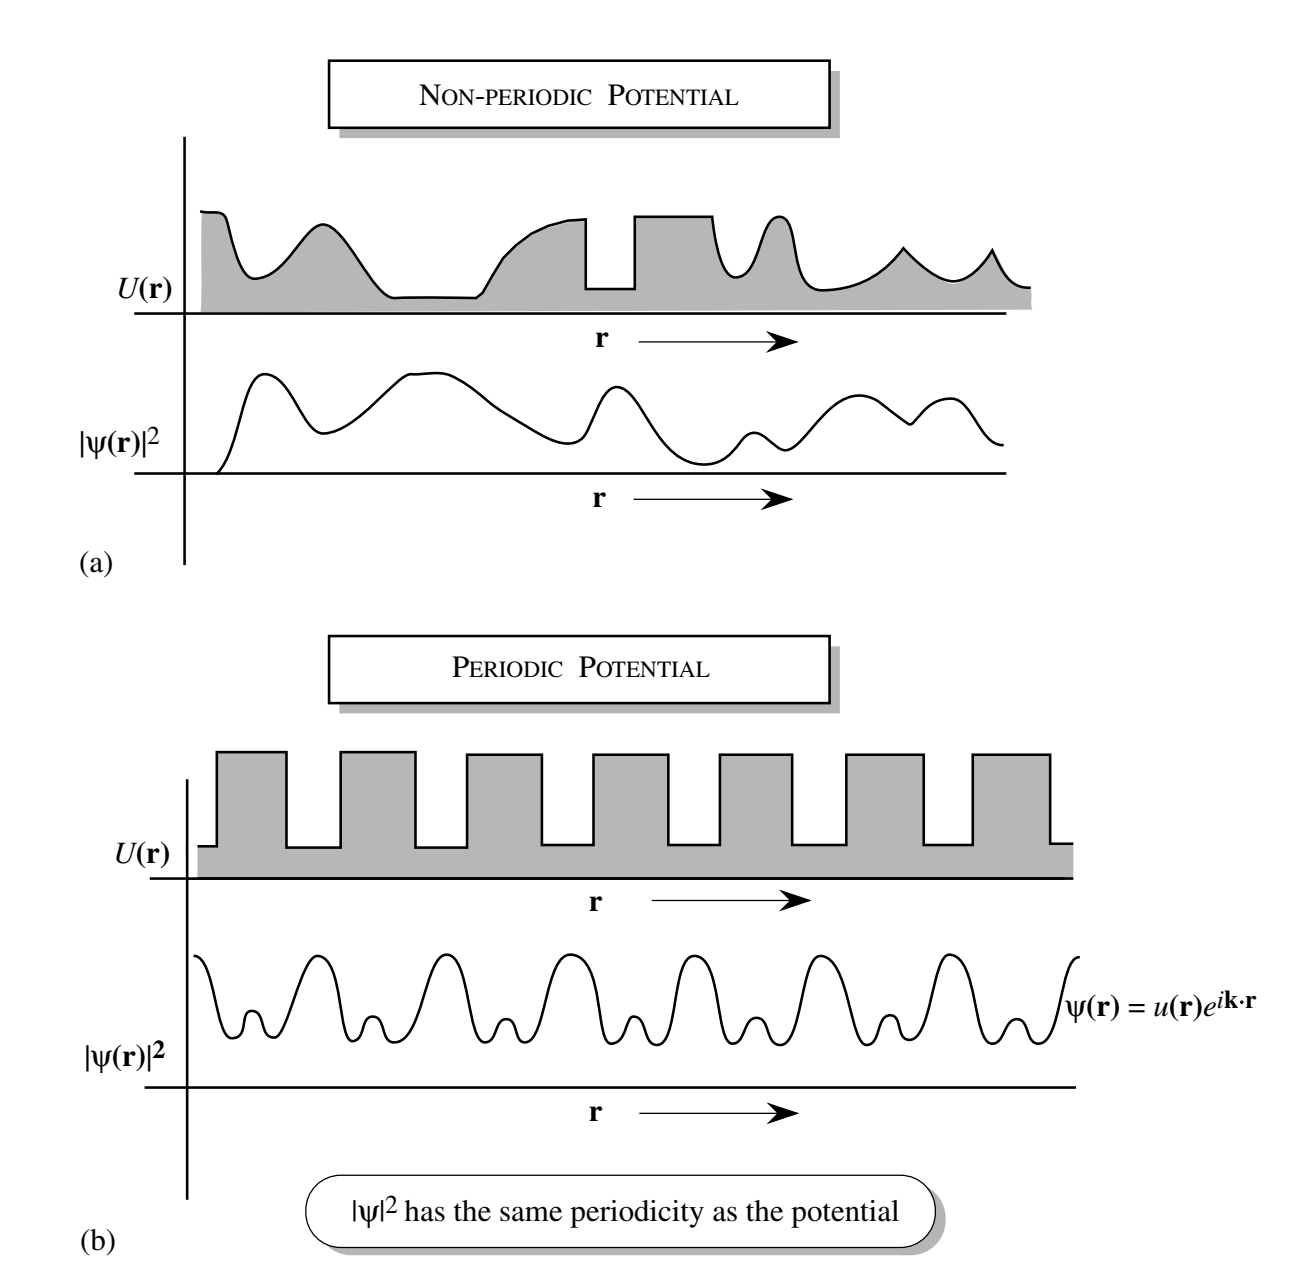
\includegraphics[width=\textwidth]{img/periodic_potential.png}
		\\[0.5em]
		\refstepcounter{figure}
		\textbf{Figure~\thefigure.} (a) Example of an electronic wavefunction in a disordered material. (b) In a periodic potential, \( |\psi|^2 \) shares the same periodicity, as required by Bloch's theorem.
		\label{fig:periodic_potential}
	\end{minipage}
\end{center}
This implies that the full wavefunction transforms under lattice translations as:
\begin{equation*}
	\psi_{\mathbf{k}}(\mathbf{r} + \mathbf{R}) = u_{\mathbf{k}}(\mathbf{r} + \mathbf{R}) e^{i\mathbf{k} \cdot (\mathbf{r} + \mathbf{R})} = u_{\mathbf{k}}(\mathbf{r}) e^{i\mathbf{k} \cdot \mathbf{r}} e^{i\mathbf{k} \cdot \mathbf{R}} = \psi_{\mathbf{k}}(\mathbf{r}) e^{i\mathbf{k} \cdot \mathbf{R}}
\end{equation*}
The vector \( \mathbf{k} \), known as the wavevector or \( \mathbf{k} \)-vector, is fundamental in describing the electronic properties of crystalline solids.

\subsection{Significance of the k-Vector}
One of the key consequences of Bloch's theorem is that, in a perfectly periodic potential provided by the crystal lattice, electrons can propagate through the material without experiencing scattering. In such a scenario, the electron wavefunction, which resembles \( \sim e^{i\mathbf{k} \cdot \mathbf{r}} \), describes an extended state that spans the entire crystal.
To understand how electrons behave under external influences, we seek to derive an equation of motion that captures their response to external forces. Let \( \mathbf{F}_{\text{ext}} \) denote an external force acting on the electron, and \( \mathbf{F}_{\text{int}} \) represent the internal force arising from the atomic lattice. Newton’s second law can then be expressed as:
\begin{equation*}
	\frac{d\mathbf{p}}{dt} = \mathbf{F}_{\text{ext}} + \mathbf{F}_{\text{int}}
\end{equation*}
\noindent However, this form is not particularly useful, as it involves the internal forces, which are typically complex to evaluate. To describe the electron's motion more effectively, we need an equation that depends solely on the external forces. We now outline a simplified derivation of such an expression, which also helps clarify the physical interpretation of the wavevector \( \mathbf{k} \) introduced in Bloch’s theorem.
Starting from the time-dependent Schrödinger equation, the general solution for electrons in a periodic potential can be written as:
\begin{equation*}
	\psi(\mathbf{r}, t) = u_{\mathbf{k}}(\mathbf{r}) e^{i(\mathbf{k} \cdot \mathbf{r} - \omega t)}
\end{equation*}
\noindent where the energy of the electron is connected to the angular frequency \( \omega \) by the relation:
\begin{equation*}
	E = \hbar \omega
\end{equation*}
\noindent The Bloch function thus corresponds to a plane wave that extends throughout the crystalline solid. To describe a spatially localized electron, we consider a wavepacket composed of Bloch states centered around a specific wavevector \( \mathbf{k} \). The group velocity of this wavepacket is given by:
\begin{equation*}
	\mathbf{v}_g = \frac{d\omega}{d\mathbf{k}} = \frac{1}{\hbar} \frac{dE}{d\mathbf{k}} = \frac{1}{\hbar} \nabla_{\mathbf{k}} E(\mathbf{k})
\end{equation*}

In the presence of an electric field \( \mathbf{F} \), the energy gained by the electron over a short time interval \( \delta t \) is:
\begin{equation*}
	\delta E = -e \mathbf{F} \cdot \mathbf{v}_g \, \delta t
\end{equation*}
\noindent More generally, the change in energy can be expressed as:
\begin{equation*}
	\delta E = \frac{dE}{d\mathbf{k}} \cdot \delta \mathbf{k} = \hbar \mathbf{v}_g \cdot \delta \mathbf{k}
\end{equation*}
\noindent Equating the two expressions for \( \delta E \), we obtain:
\begin{equation*}
	\delta \mathbf{k} = -\frac{e \mathbf{F}}{\hbar} \delta t
\end{equation*}
\noindent which leads to the equation of motion for the wavevector:
\begin{equation*}
	\hbar \frac{d\mathbf{k}}{dt} = -e \mathbf{F}
\end{equation*}
\noindent Since \( -e\mathbf{F} \) is the force acting on the electron, this can be generalized to:
\begin{equation*}
	\hbar \frac{d\mathbf{k}}{dt} = \mathbf{F}_{\text{ext}}
\end{equation*}
\noindent This result mirrors Newton’s second law:
\begin{equation*}
	\frac{d\mathbf{p}}{dt} = \mathbf{F}_{\text{ext}}
\end{equation*}
\noindent provided we identify \( \hbar d\mathbf{k} \) with the momentum of the electron inside the crystal. While \( \hbar d\mathbf{k} \) behaves as the momentum in response to external forces, it is not the true mechanical momentum since it incorporates the effects of the internal periodic potential. Instead, \( \hbar \mathbf{k} \) is referred to as the \textit{crystal momentum}.

\section{Metals, Insulators, and Semiconductors}
From atomic physics, it is known that bound electrons occupy discrete energy levels, separated by regions where no states exist. In solids, these discrete levels broaden into continuous energy bands, with forbidden gaps—bandgaps—separating them. Once the electronic band structure is known, a key question arises: which of the available states are occupied by electrons, and which remain empty?
Two important cases emerge regarding electron occupation: in one scenario, an energy band is fully occupied at 0~K, while the next higher band is separated by an energy gap \( E_g \) and remains completely unoccupied. In the second case, the highest energy band that contains electrons is only partially filled.
At this stage, a critical concept must be introduced. When an energy band is completely filled, the electrons within it cannot contribute to electrical conduction. This is a direct consequence of the Pauli exclusion principle: since electrons are fermions, they can only transition into unoccupied states. In a filled band, all such states are already occupied, leading to a cancellation of net motion—electrons moving in opposite directions balance each other. As a result, materials with fully filled bands and an energy gap above them exhibit, in principle, infinite resistivity and are classified as insulators or semiconductors.
In contrast, if the highest occupied band is only partially filled, available empty states exist within the same band. This allows electrons to accelerate under an external field, enabling electrical conduction. Such materials exhibit low resistivity and are termed metals.
\begin{center}
	\begin{minipage}{0.6\textwidth}
		\centering
		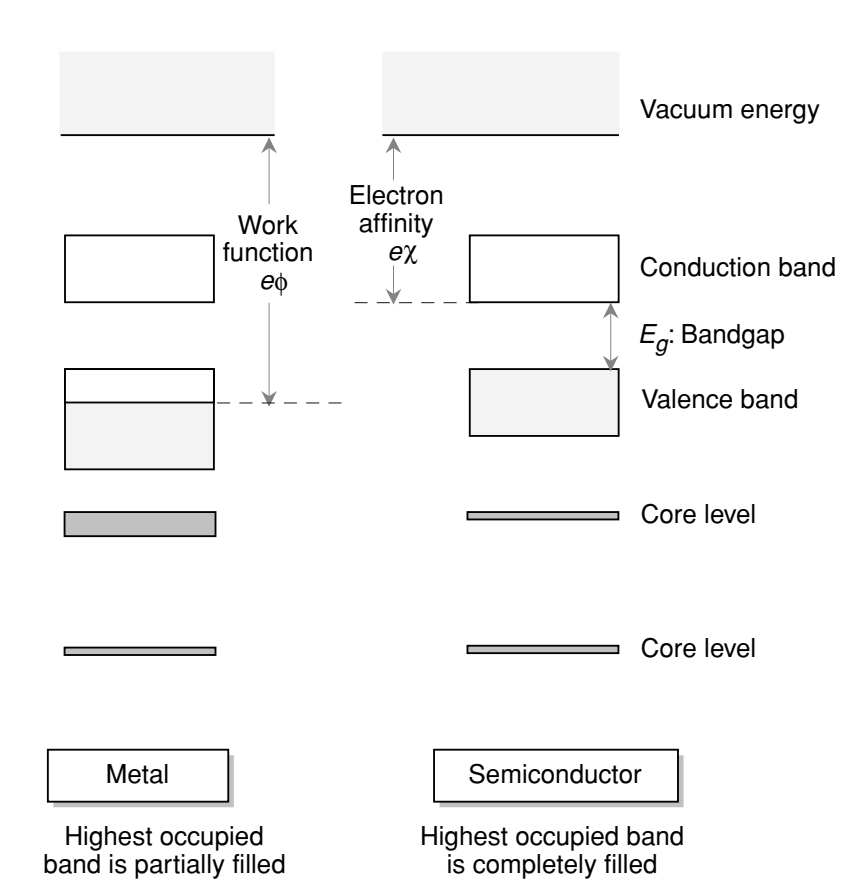
\includegraphics[width=\textwidth]{img/metalsVSsemiconductors.png}
		\\[0.5em]
		\refstepcounter{figure}
		\textbf{Figure~\thefigure.} Band occupation at 0~K for a metal and a semiconductor. In metals, the top band is partially filled. In semiconductors, the valence band is full and separated from the empty conduction band by the bandgap \( E_g \). Work function and electron affinity are indicated.
		\label{fig:metalsVSsemiconductors}
	\end{minipage}
\end{center}
The band that is fully occupied by electrons at absolute zero in semiconductors is known as the \textit{valence band}, whereas the higher energy band that remains empty at 0~K is referred to as the \textit{conduction band}. In metals, the energy difference between the vacuum level and the highest occupied electronic state is termed the \textit{work function}. For semiconductors, the energy separating the vacuum level from the bottom of the conduction band is called the \textit{electron affinity}.
Metals are characterized by extremely high electrical conductivity, resulting from the large number of electrons available for conduction. However, this abundance of charge carriers also makes it difficult to significantly modify their conductivity. Semiconductors, in contrast, exhibit zero conductivity at 0~K and relatively low conductivity at finite temperatures. Importantly, their conductivity can be altered dramatically—by several orders of magnitude—which is the foundation of their utility in active electronic components.
As previously discussed, semiconductors are defined as materials in which the valence band is completely filled and the conduction band completely empty at 0~K. When the temperature is raised above absolute zero, some electrons gain enough thermal energy to transition from the valence band into the conduction band. This results in the creation of empty states (holes) in the valence band and free electrons in the conduction band.
When electrons are thermally excited into the conduction band, the valence band is left with some unoccupied states. Consider the situation illustrated in the scheme below, where an electron with wavevector \( \mathbf{k}_e \) is missing from the valence band. In a completely filled valence band, the total sum over all electron wavevectors is zero:

\begin{equation*}
	\sum_i \mathbf{k}_i = \sum_{\mathbf{k}_e} \mathbf{k}_e + \sum_{-\mathbf{k}_e} (-\mathbf{k}_e) = 0
\end{equation*}
\noindent
This simply reflects the fact that for every occupied positive wavevector state, there exists a corresponding occupied state with a negative wavevector.

Now, when an electron is missing from a particular state \( \mathbf{k}_e \), the net wavevector of the system becomes:
\begin{equation*}
	\mathbf{k}_h = -\mathbf{k}_e
\end{equation*}
\noindent
This unoccupied state is referred to as a \textit{hole}, and the wavevector \( -\mathbf{k}_e \) is attributed to it. Although the missing electron originated from the state \( \mathbf{k}_e \), the hole is described as having wavevector \( \mathbf{k}_h = -\mathbf{k}_e \), as illustrated. The hole's position corresponds to where the electron would have been.

It is important to emphasize that a hole represents the absence of an electron in the valence band. When the valence band is completely filled, it cannot contribute to electrical conduction. However, once an electron is removed, current can flow. Under the application of an electric field, electrons drift in the direction opposite to the field, which effectively causes the unoccupied (hole) state to move in the direction of the field. Thus, the hole behaves like a positively charged particle.

\begin{center}
	\begin{minipage}{0.7\textwidth}
		\centering
		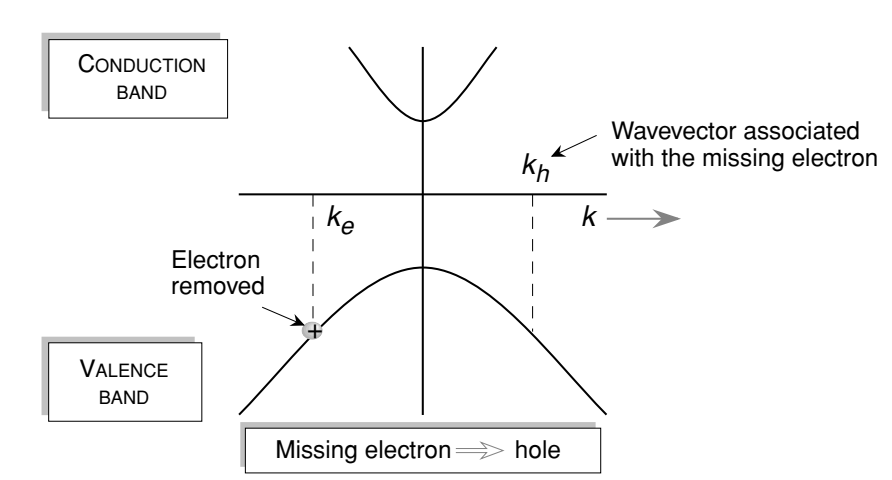
\includegraphics[width=\textwidth]{img/missingelectron.png}
		\\[0.5em]
		\refstepcounter{figure}
		\textbf{Figure~\thefigure.} Illustration of a the wavector of the missng electron $\mathbf{k}_e$ and the corresponding hole wavevector $-\mathbf{k}_e$.
		\label{fig:missingelectron}
	\end{minipage}
\end{center}

The response of the hole to electric and magnetic fields \( \mathbf{F} \) and \( \mathbf{B} \) is described by the following equation of motion:
\begin{equation*}
	\hbar \frac{d\mathbf{k}_h}{dt} = e\left[\mathbf{F} + \mathbf{v}_h \times \mathbf{B} \right]
\end{equation*}
\noindent
where \( \hbar \mathbf{k}_h \) is the crystal momentum of the hole and \( \mathbf{v}_h \) is its velocity.

\section{Tight-Binding Method}
Before delving into the properties of various semiconductors, it is helpful to first examine the atomic structure of the constituent elements.

\subsection*{Group IV Semiconductors}

\begin{itemize}
	\item \textbf{C:} \quad 1s$^2$ 2s$^2$ 2p$^2$
	\item \textbf{Si:} \quad 1s$^2$ 2s$^2$ 2p$^6$ 3s$^2$ 3p$^2$
	\item \textbf{Ge:} \quad 1s$^2$ 2s$^2$ 2p$^6$ 3s$^2$ 3p$^6$ 3d$^{10}$ 4s$^2$ 4p$^2$
\end{itemize}

\subsection*{Group III–V Semiconductors}

\begin{itemize}
	\item \textbf{Ga:} \quad 1s$^2$ 2s$^2$ 2p$^6$ 3s$^2$ 3p$^6$ 3d$^{10}$ 4s$^2$ 4p$^1$
	\item \textbf{As:} \quad 1s$^2$ 2s$^2$ 2p$^6$ 3s$^2$ 3p$^6$ 3d$^{10}$ 4s$^2$ 4p$^3$
\end{itemize}

A key observation from these configurations is that the valence electrons in all relevant semiconductor elements occupy either $s$- or $p$-type orbitals. While this is true for isolated atoms, it also holds in crystalline solids: electrons in the valence and conduction bands retain this $s$- or $p$-like orbital character, even though they become delocalized as Bloch states. This feature plays a fundamental role in determining the optical and transport behavior of semiconductors.

\subsection*{Bandstructure and the Tight Binding Method}

We now turn to techniques for calculating the bandstructure of materials. As previously noted, there are both comprehensive methods and those valid only near specific energy ranges. We begin with the \textit{tight binding method} (TBM), an empirical approach that uses experimental data to model the bandstructure.

In TBM, atomic orbitals are used as the basis for constructing Bloch functions. The periodic part of the Bloch wavefunction is written as a linear combination of atomic orbitals centered on the crystal lattice sites. If \( \phi(\mathbf{r} - \mathbf{R}) \) represents an atomic orbital centered at position \( \mathbf{R} \), the Bloch wavefunction can be expressed as:
\begin{equation*}
	\psi_{n\mathbf{k}}(\mathbf{r}) = \sum_{\mathbf{R}_n} \phi_n(\mathbf{r} - \mathbf{R}) \exp(i\mathbf{k} \cdot \mathbf{R_n})
\end{equation*}

The periodic part of the Block Function is expanded in terms of the atomic-like orbitals of the atoms of the unit cell (index \textit{n} in the summation).

As mentioned, the outermost electrons in the semiconductor elements are associated with $s$- and $p$-type orbitals. While core electrons do not significantly contribute to band formation, the valence orbitals do. When atoms are brought together to form a solid, these discrete atomic states broaden into energy bands. Although the atomic orbitals are no longer exact eigenstates in the crystal, they serve as an excellent approximate basis for describing the electronic states.\\
This forms the central idea of the tight binding model. We start from the known atomic solutions, which satisfy:
\begin{equation*}
	H_\text{at} \psi_n = E_n \psi_n
\end{equation*}
The goal is to construct approximate Bloch-like states from these atomic solutions:
\begin{equation*}
	\psi_{\mathbf{k}}(\mathbf{r}) = \sum_{n,\mathbf{R}} e^{i\mathbf{k} \cdot \mathbf{R}} \psi_n(\mathbf{r} - \mathbf{R})
\end{equation*}

However, these states do not account for the interactions between atoms in the crystal. To include this effect, we consider the total crystal Hamiltonian as:
\begin{equation*}
	H_\text{cryst} = H_\text{at} + \Delta U(\mathbf{r})
\end{equation*}

Here, \( \Delta U(\mathbf{r}) \) represents the additional potential arising from neighboring atoms—this is what perturbs the atomic states and causes band formation.
\begin{center}
	\begin{minipage}{0.9\textwidth}
		\centering
		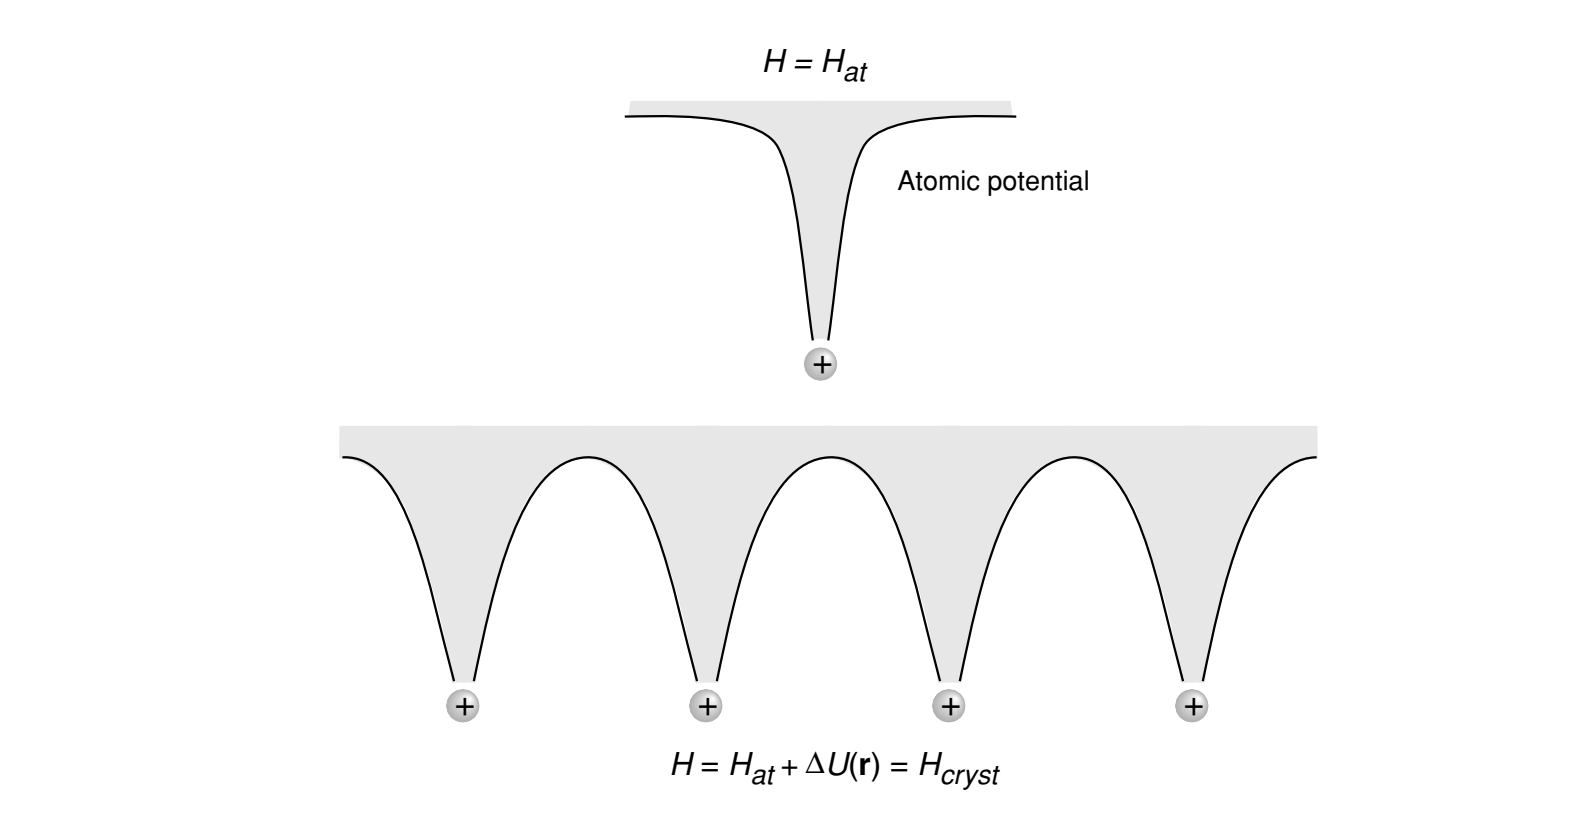
\includegraphics[width=\textwidth]{img/neighboring_atoms.png}
		\\[0.5em]
		\refstepcounter{figure}
		\textbf{Figure~\thefigure.} The effect of neighboring atoms is to perturb the atomic states, leading to the formation of bands. The perturbation is represented by \( \Delta U(\mathbf{r}) \).
		\label{fig:neighboring_atoms}
	\end{minipage}
\end{center}

The new wavefunctions must respect Bloch’s theorem and can be written in the general form:
\begin{equation}
	\Psi_{\mathbf{k}}(\mathbf{r}) = \sum_{\mathbf{R}} e^{i\mathbf{k} \cdot \mathbf{R}} \phi(\mathbf{r} - \mathbf{R})
	\label{eq:bloch_wavefunction}
\end{equation}
In this context, the function \( \phi(\mathbf{r}) \) is not itself an atomic orbital but is instead constructed as a linear combination of atomic eigenfunctions. Specifically, we can express \( \phi(\mathbf{r}) \) in terms of a finite set of atomic orbitals \( \psi_n(\mathbf{r}) \) as:
\begin{equation}
	\phi(\mathbf{r}) = \sum_{n=1}^{N} b_n \psi_n(\mathbf{r})
	\label{eq:linear_combination}
\end{equation}

\noindent
Here, \( N \) is the number of atomic orbitals included in the basis, and \( b_n \) are coefficients to be determined. In the tight binding method, only a limited number \( N \) of orbitals are retained for computational tractability.

To determine the coefficients \( b_n \), we substitute the equation above into the time-independent Schrödinger equation and derive a system of \( N \) coupled equations by projecting onto the atomic basis set. The Schrödinger equation for the crystal takes the form:
\begin{equation}
	H\Psi_{\mathbf{k}} = E(\mathbf{k}) \Psi_{\mathbf{k}}
	\label{eq:schrodinger_crystal}
\end{equation}

\noindent
Substituting Eq.\eqref{eq:bloch_wavefunction} and Eq.\eqref{eq:linear_combination}  into Eq.\eqref{eq:schrodinger_crystal}, multiplying from the left by \( \psi_m^*(\mathbf{r}) \), and integrating over all space gives:
\begin{equation}
	\int d^3 r \, \psi_m^*(\mathbf{r}) \left\{
	\left[ H_{\text{at}} + \Delta U(\mathbf{r}) \right]
	\sum_{\mathbf{R},n} b_n \, e^{i \mathbf{k} \cdot \mathbf{R}} \, \psi_n(\mathbf{r} - \mathbf{R})
	- E(\mathbf{k}) \sum_{\mathbf{R},n} b_n \, e^{i \mathbf{k} \cdot \mathbf{R}} \, \psi_n(\mathbf{r} - \mathbf{R})
	\right\} = 0
\end{equation}

\noindent
Since the atomic orbitals are orthonormal when centered on the same atom, we have:
\begin{equation}
	\int d^3r \, \psi_m^*(\mathbf{r}) \psi_n(\mathbf{r}) = \delta_{mn}
\end{equation}

\noindent
However, this orthogonality does not generally hold when the orbitals are centered at different lattice sites. That is:
\begin{equation}
	\int d^3r \, \psi_m^*(\mathbf{r}) \psi_n(\mathbf{r} - \mathbf{R}) \neq \delta_{mn} \quad \text{for} \quad \mathbf{R} \ne 0
\end{equation}

\noindent
This non-orthogonality must be accounted for in the tight binding formalism and leads to overlap integrals that influence the coupling between neighboring atomic orbitals.

In the summation over lattice vectors, we separate the terms with $\mathbf{R} = 0$ and $\mathbf{R} \neq 0$ to get,
\begin{align*}
	 & (E(\mathbf{k}) - E_m) b_m =                                                                                                                                                                           \\
	 & -(E(\mathbf{k}) - E_m) \sum_{n=1}^{N} \left( \sum_{\mathbf{R} \neq 0} \int \psi_m^*(\mathbf{r}) \, \psi_n(\mathbf{r} - \mathbf{R}) \, e^{i \mathbf{k} \cdot \mathbf{R}} \, d^3 r \right) b_n \notag   \\
	 & \quad + \sum_{n=1}^{N} \left( \int \psi_m^*(\mathbf{r}) \, \Delta U(\mathbf{r}) \, \psi_n(\mathbf{r}) \, d^3 r \right) b_n \notag                                                                     \\
	 & \quad + \sum_{n=1}^{N} \left( \sum_{\mathbf{R} \neq 0} \int \psi_m^*(\mathbf{r}) \, \Delta U(\mathbf{r}) \, \psi_n(\mathbf{r} - \mathbf{R}) \, e^{i \mathbf{k} \cdot \mathbf{R}} \, d^3 r \right) b_n
\end{align*}

It is important to recognize the use of the identity:
\begin{equation}
	\int d^3r \, \psi_m^*(\mathbf{r}) H_{\text{at}} \psi_n(\mathbf{r}) = E_m \delta_{mn}
\end{equation}

\noindent
where \( E_m \) is the energy eigenvalue associated with the atomic orbital \( \psi_m \). Note that these energies \( E_m \) may not exactly correspond to the isolated atomic energy levels, since the presence of neighboring atoms in the crystal modifies them. As such, in the tight binding method, these energies are often treated as fitting parameters to match experimental data or more accurate calculations.

An additional approximation typically made in the tight binding framework is:
\begin{equation}
	\int d^3r \, \psi_m^*(\mathbf{r}) \psi_n(\mathbf{r} - \mathbf{R}) e^{i\mathbf{k} \cdot \mathbf{R}} \approx 0
\end{equation}

\noindent
This implies that the spatial overlap between atomic orbitals centered on different atoms is negligible, which is valid when the atomic orbitals are strongly localized.

Another important concept is the \textit{on-site matrix element}, defined as:
\begin{equation}
	\int d^3r \, \psi_m^*(\mathbf{r}) H \psi_n(\mathbf{r}) = E_m + \int d^3r \, \psi_m^*(\mathbf{r}) \Delta U(\mathbf{r}) \psi_m(\mathbf{r})
\end{equation}

\noindent
For many forms of the potential \( \Delta U(\mathbf{r}) \), the integral:
\begin{equation}
	\int d^3r \, \psi_m^*(\mathbf{r}) \Delta U(\mathbf{r}) \psi_n(\mathbf{r})
\end{equation}

\noindent
vanishes when \( m \neq n \), which further simplifies the matrix elements.

To obtain the eigenvalues \( E(\mathbf{k}) \) and corresponding eigenfunctions (with coefficients \( b_n \)), we solve a system of \( N \) coupled linear equations. These form an \( N \times N \) \textit{secular equation}, from which the energy dispersion \( E(\mathbf{k}) \), or the bandstructure, can be determined. For each wavevector \( \mathbf{k} \), the solution yields \( N \) energy levels, corresponding to the bands derived from the \( N \) atomic orbitals used in the basis.

To gain intuition about this method, we next examine a simple case involving only $s$-orbitals—a so-called \textit{s-band model}.

\subsection{Tight Binding Model for s-Bands}
In the case of semiconductors, each unit cell typically contains two atoms in the basis. For each atom, it is necessary to include at least the outer shell orbitals: one \(s\)-orbital and three \(p\)-orbitals (\(p_x\), \(p_y\), and \(p_z\)). As a result, the tight binding secular equation becomes significantly more complex due to the increased number of basis functions.

To gain some intuitive understanding, we now consider a simplified model: a crystal with a single atom per unit cell and only one orbital per atom—the \(s\)-orbital. In this scenario, there is only one atomic level, and all tight binding coefficients \( \{b_n\} \) are zero except for the \(s\)-level, where \( b_s = 1 \). This simplification reduces the problem to a single equation.

We obtain:
\begin{align*}
	E(k) - E_s = & - (E(k) - E_s) \sum_{\mathbf{R} \neq 0} \int d^3r \, \psi_s^*(\mathbf{r}) \psi_s(\mathbf{r} - \mathbf{R}) e^{i\mathbf{k} \cdot \mathbf{R}}         \\
	             & + \int d^3r \, \psi_s^*(\mathbf{r}) \Delta U(\mathbf{r}) \psi_s(\mathbf{r})                                                                        \\
	             & + \sum_{\mathbf{R} \neq 0} \int d^3r \, \psi_s^*(\mathbf{r}) \Delta U(\mathbf{r}) \psi_s(\mathbf{r} - \mathbf{R}) e^{i\mathbf{k} \cdot \mathbf{R}}
\end{align*}
We define the following integrals to simplify notation:
\begin{align}
	\boxed{
		\alpha(\mathbf{R}) = \int d^3r \, \psi_s^*(\mathbf{r}) \psi_s(\mathbf{r} - \mathbf{R})
	} \\[8pt]
	\boxed{
		\beta_s = -\int d^3r \, \psi_s^*(\mathbf{r}) \Delta U(\mathbf{r}) \psi_s(\mathbf{r})
	} \\[8pt]
	\overset{\text{HOPPING INTEGRAL} \,}{\boxed{
			\gamma(\mathbf{R}) = -\int d^3r \, \psi_s^*(\mathbf{r}) \Delta U(\mathbf{r}) \psi_s(\mathbf{r} - \mathbf{R})
		}}
\end{align}

As discussed earlier, we typically neglect the overlap integral \( \alpha(\mathbf{R}) \), i.e., we set \( \alpha(\mathbf{R}) = 0 \), assuming strong localization of atomic orbitals. The energy dispersion relation simplifies to:
\begin{equation}
	\boxed{
		E(\mathbf{k}) = E_s - \beta - \sum_{\mathbf{R}} \gamma(\mathbf{R}) e^{i\mathbf{k} \cdot \mathbf{R}}}
\end{equation}
The off-site matrix elements \( \gamma(\mathbf{R}) \) decay rapidly with increasing distance \( \mathbf{R} \), so we consider only the nearest-neighbor interactions. Additionally, due to lattice symmetry, \( \gamma(-\mathbf{R}) = \gamma(\mathbf{R}) \).

Let us now apply this to a face-centered cubic (fcc) lattice. The twelve nearest neighbors of a lattice site in an fcc crystal are located at:
\begin{equation*}
	\frac{a}{2} (\pm1, \pm1, 0), \quad \frac{a}{2} (\pm1, 0, \pm1), \quad \frac{a}{2} (0, \pm1, \pm1)
\end{equation*}
Taking into account all twelve neighbors, the energy becomes:
\begin{align*}
	E(\mathbf{k}) & = E_s - \beta - \gamma \sum_{\mathbf{R}} e^{i\mathbf{k} \cdot \mathbf{R}}                                                                                                                                                                                \\
	              & = E_s - \beta - \boxed{4\gamma} \left[ \cos\left(\frac{k_x a}{2}\right) \cos\left(\frac{k_y a}{2}\right) + \cos\left(\frac{k_y a}{2}\right) \cos\left(\frac{k_z a}{2}\right) + \cos\left(\frac{k_z a}{2}\right) \cos\left(\frac{k_x a}{2}\right) \right]
\end{align*}
This final expression captures \textbf{the energy dispersion relation} for an \(s\)-band in an fcc lattice, considering only nearest-neighbor interactions.

We now analyze the energy band derived above within the context of the first Brillouin zone of the face-centered cubic (fcc) lattice.
From the geometry of the Brillouin zone, we observe that there are six equivalent \( X \)-points and eight equivalent \( L \)-points, which are critical in determining the behavior of the electronic bandstructure.\\
By evaluating the energy expression from the last relation obtained along various high-symmetry directions in \( \mathbf{k} \)-space, we can obtain the band dispersion throughout the Brillouin zone. The resulting energy bands reflect the symmetry of the lattice and provide insight into the electronic properties of the material.
\begin{center}
	\begin{minipage}{0.9\textwidth}
		\centering
		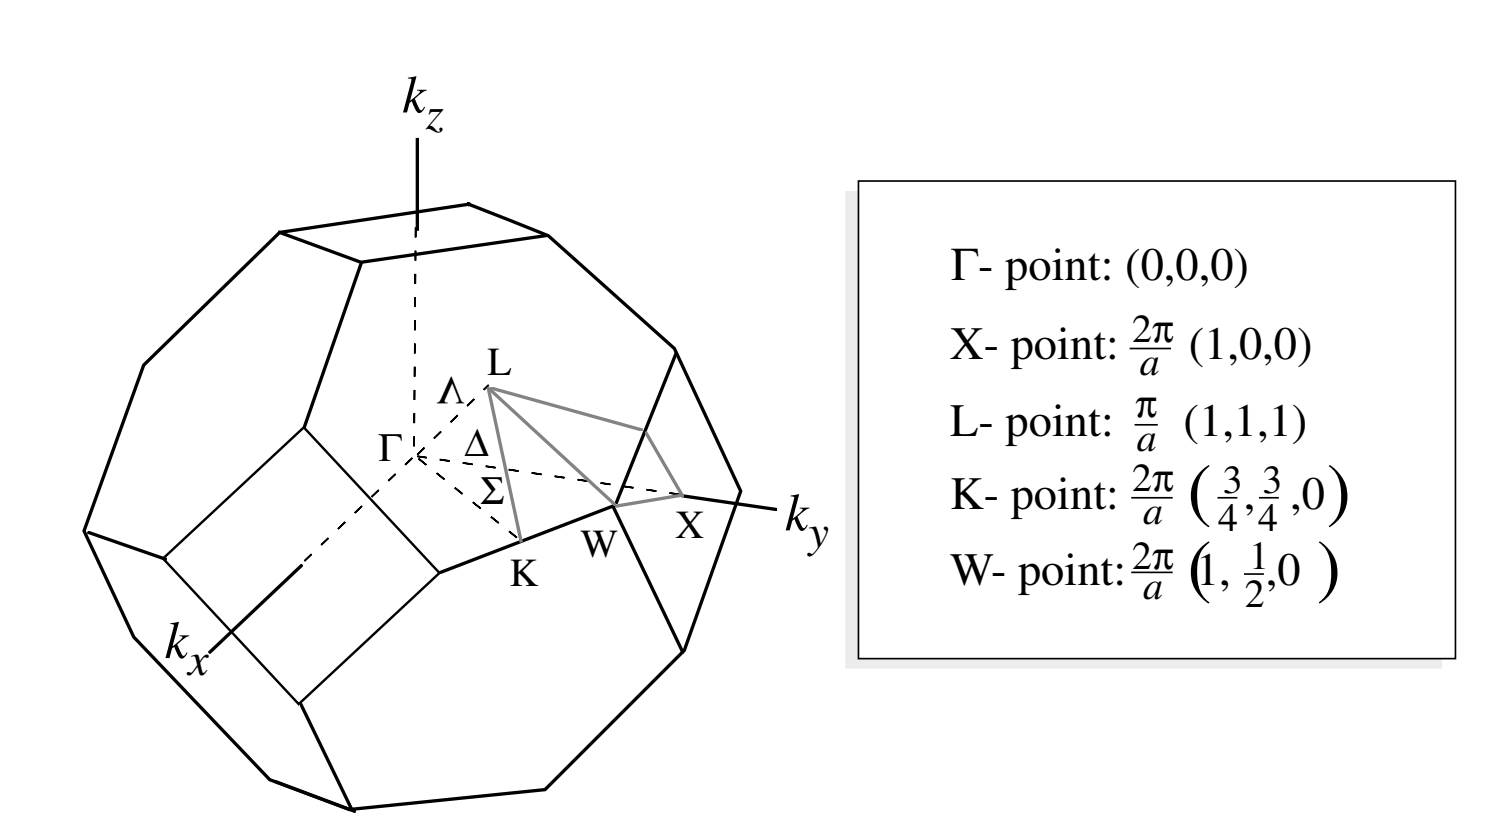
\includegraphics[width=\textwidth]{img/BrillouinZones.png}
		\\[0.5em]
		\refstepcounter{figure}
		\textbf{Figure~\thefigure.} Brillouin zones of the face-centered cubic (fcc) lattice. The high-symmetry points \( \Gamma \), \( X \), and \( L \) are indicated, along with their corresponding coordinates in reciprocal space.
		\label{fig:BrillouinZones}
	\end{minipage}
\end{center}

To further understand the nature of the bandstructure, we examine the dispersion relation \( E(\mathbf{k}) \) along key high-symmetry directions in the first Brillouin zone of the fcc lattice. These paths correspond to the directions \( \Gamma \rightarrow X \), \( \Gamma \rightarrow L \), and \( \Gamma \rightarrow K \), and the corresponding energy expressions can be obtained by substituting specific components of \( \mathbf{k} \) into Eq.~(2.35).

\begin{itemize}
	\item \textbf{Along \( \Gamma X \)}: Set \( k_x = \frac{2\pi \alpha}{a} \), \( k_y = k_z = 0 \), with \( 0 \leq \alpha \leq 1 \). The energy becomes:
	      \begin{equation*}
		      E(\mathbf{k}) = E_s - \beta - 4\gamma (1 + 2 \cos \pi \alpha)
	      \end{equation*}
	\item \textbf{Along \( \Gamma L \)}: Set \( k_x = k_y = k_z = \frac{2\pi \alpha}{a} \), with \( 0 \leq \alpha \leq \frac{1}{2} \). The energy expression is:
	      \begin{equation*}
		      E(\mathbf{k}) = E_s - \beta - 12\gamma \cos^2(\pi \alpha)
	      \end{equation*}
	\item \textbf{Along \( \Gamma K \)}: Set \( k_x = k_y = \frac{2\pi \alpha}{a} \), \( k_z = 0 \), with \( 0 \leq \alpha \leq \frac{3}{4} \). The energy becomes:
	      \begin{equation*}
		      E(\mathbf{k}) = E_s - \beta - 4\gamma \left( \cos^2 \pi \alpha + 2 \cos\left( \frac{\pi \alpha}{2} \right) \right)
	      \end{equation*}
\end{itemize}

The bandstructure—i.e., the relation between energy \( E \) and wavevector \( \mathbf{k} \)—is typically plotted along these high-symmetry paths, as shown in Fig.\ref{fig:BrillouinZones}. In the illustrative case where \( \gamma = 1.0\,\text{eV} \) and \( E_s + \beta = 0 \), the resulting bandwidth is found to be:
\begin{equation*}
	\Delta E = 16\gamma
\end{equation*}
This shows that greater overlap between neighboring atomic orbitals (i.e., larger \( \gamma \)) leads to wider energy bands.
It is particularly useful to analyze the bandstructure near the \( \Gamma \) point, where the wavevector \( \mathbf{k} \) is small. By choosing \( k_x = k_y = k_z = k/\sqrt{3} \) such that \( ka \ll 1 \), the cosine terms can be expanded, yielding:
\begin{equation}
	E(\mathbf{k}) = E_s - \beta - 12\gamma + \gamma a^2 k^2
\end{equation}
Comparing this expression with the free electron dispersion relation:
\begin{equation*}
	E(p) = E_0 + \frac{p^2}{2m}
\end{equation*}
\noindent
we can rewrite the tight binding result in a similar form:
\begin{equation*}
	E(\mathbf{k}) = E_s - \beta - 12\gamma + \frac{\hbar^2 k^2}{2 m^*}
\end{equation*}
This allows us to define an effective mass \( m^* \) for the electrons near the bottom of the band:
\begin{equation}
	m^* = \frac{\hbar^2}{2\gamma a^2}
\end{equation}
\noindent
This effective mass characterizes the curvature of the band near \( \Gamma \) and plays a central role in transport phenomena in semiconductors.
\begin{center}
	\begin{minipage}{0.6\textwidth}
		\centering
		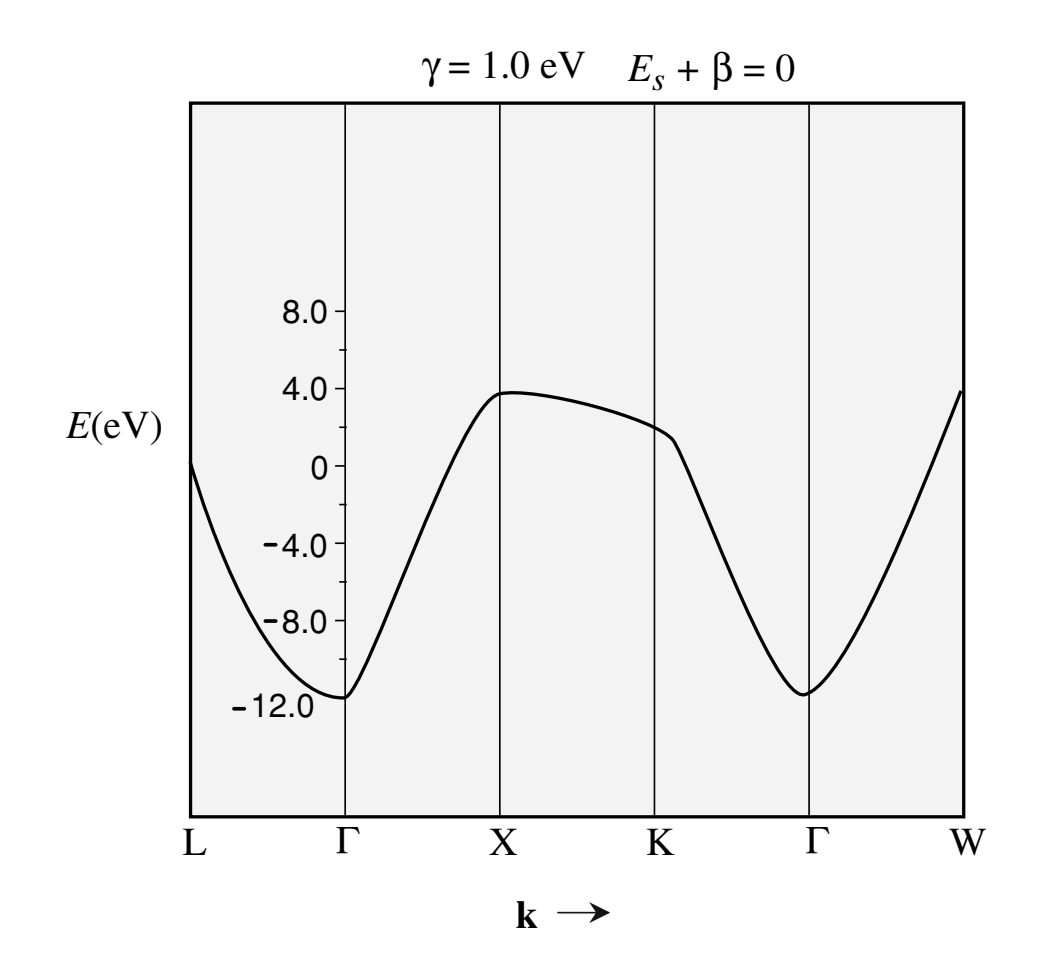
\includegraphics[width=\textwidth]{img/s-band-model.png}
		\\[0.5em]
		\refstepcounter{figure}
		\textbf{Figure~\thefigure.} Bandstructure of an \(s\)-band in a face-centered cubic (fcc) lattice. The energy dispersion is plotted along high-symmetry directions in the Brillouin zone, illustrating the relationship between energy \( E \) and wavevector \( \mathbf{k} \). The effective mass \( m^* \) is defined near the \( \Gamma \) point.
		\label{fig:s-band-model}
	\end{minipage}
\end{center}


\subsection{Bandstructure of Semiconductors}
We now extend the discussion of TBM to semiconductor materials. As previously mentioned, the outermost electrons in semiconductors are typically described using atomic orbitals of type \( s \), \( p_x \), \( p_y \), and \( p_z \). The accuracy of the method can be improved by including additional atomic states, though the minimal useful basis already captures much of the essential physics.

In semiconductor crystals, there are typically two atoms per unit cell. Therefore, to describe the central-cell portion of the Bloch functions, we require a total of eight atomic orbitals—four per atom. We construct the Bloch-like wavefunction as:
\begin{equation}
	\Psi(\mathbf{k}, \mathbf{r}) = \sum_{R_i} \sum_{j=1}^{2} \sum_{m=1}^{4} C_{mj}(\mathbf{k}) \, \phi_{mj}(\mathbf{r} - \mathbf{r}_j - \mathbf{R}_i) \, e^{i\mathbf{k} \cdot \mathbf{R}_i}
\end{equation}
\noindent
Here, \( \mathbf{R}_i \) runs over the lattice vectors, \( j \) indexes the atoms within each unit cell, \( m \) refers to the atomic orbital type (\( s, p_x, p_y, p_z \)), and \( \phi_{mj} \) are the atomic-like basis functions centered at position \( \mathbf{r}_j \) in the unit cell. The coefficients \( C_{mj}(\mathbf{k}) \) are to be determined by solving the Schrödinger equation.\\
As done in the simpler \( s \)-band case, we now formulate the Schrödinger equation as a matrix eigenvalue problem in the form of a secular determinant:
\begin{equation}
	\left| \langle \phi_{mj} | H - E(\mathbf{k}) | \Psi(\mathbf{k}) \rangle \right| = 0
\end{equation}
\noindent
Here, \( H \) is the crystal Hamiltonian, and the determinant must vanish for nontrivial solutions to exist.

In the tight binding method (TBM) applied to zinc–blende crystals using an \( sp^3 \) basis, the wavefunction is constructed from eight atomic orbitals: one \( s \)-orbital and three \( p \)-orbitals (\( p_x, p_y, p_z \)) for each of the two atoms in the Wigner–Seitz cell. This results in a total of eight basis functions per unit cell.\\

This formulation assumes that the bandstructure exhibits spin degeneracy—that is, each electronic state is doubly degenerate due to the presence of both spin-up and spin-down electrons. If one wishes to include the effects of spin–orbit coupling or any interaction that breaks spin degeneracy, the basis must be expanded accordingly.\\

In the tight binding approximation, the top of the valence band is predicted to be three-fold degenerate, corresponding to the degeneracy of the \( p_x \), \( p_y \), and \( p_z \) orbitals. When spin is taken into account, this degeneracy becomes six-fold, since each orbital state can have both spin-up and spin-down components.\\

However, experimental observations and more accurate theoretical models show that, in most semiconductors, the top of the valence band is actually two-fold degenerate (four-fold with spin). Additionally, there exists another band—also two-fold degenerate—that lies slightly below the valence band maximum.
These features cannot be captured by a purely non-relativistic tight binding model. To accurately reproduce this band splitting, relativistic effects must be incorporated. The interaction responsible for this splitting is known as \textit{spin–orbit coupling}, which lifts part of the degeneracy by coupling the electron's spin and orbital angular momentum.

\begin{center}
	\begin{minipage}{0.6\textwidth}
		\centering
		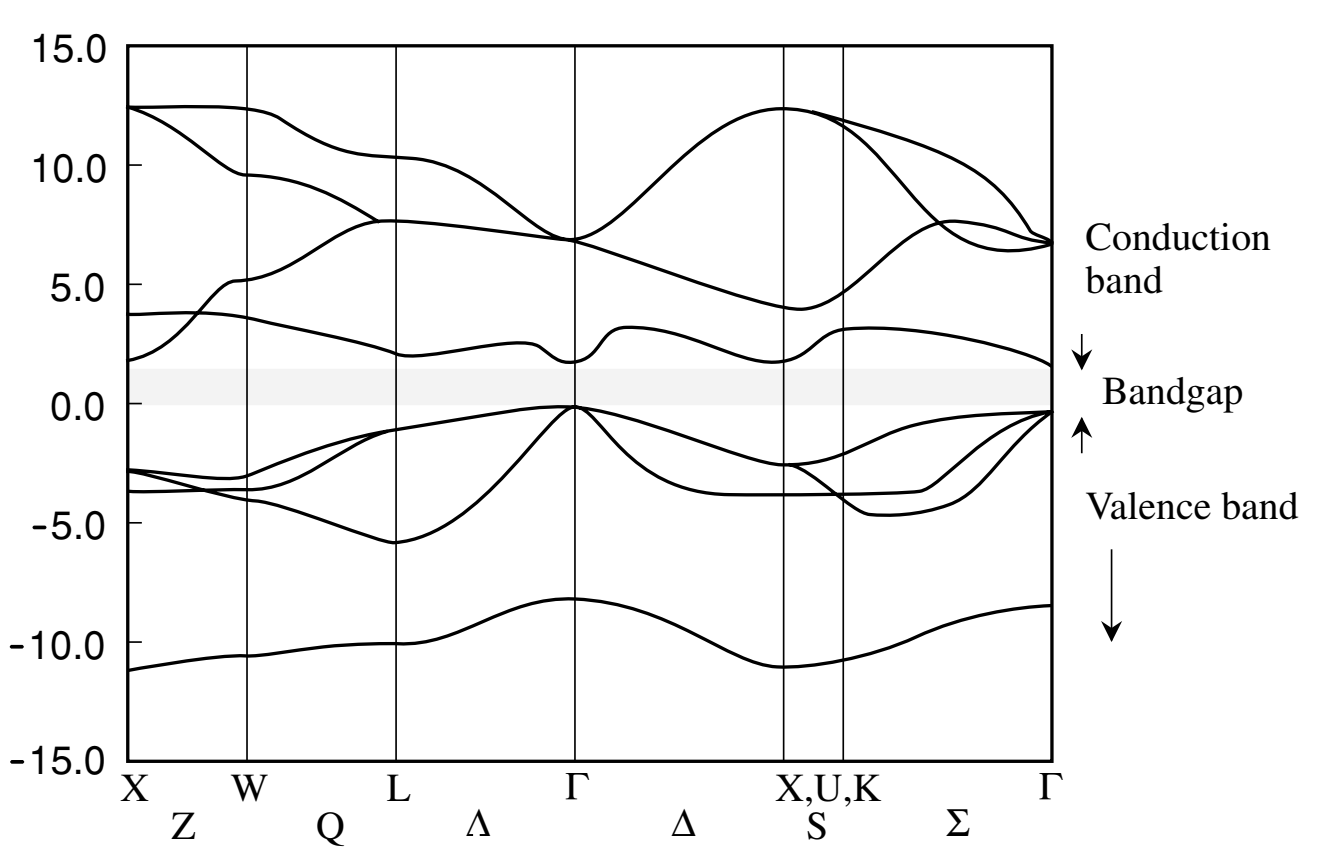
\includegraphics[width=\textwidth]{img/GaAs_TBM.png}
		\\[0.5em]
		\refstepcounter{figure}
		\textbf{Figure~\thefigure.} Band structure of GaAs obtained using the tight-binding model, excluding spin-orbit interaction. As shown, this approach alone does not provide a precise description of the valence band edge unless spin-orbit effects are taken into account.
		\label{fig:GaAs_TBM}
	\end{minipage}
\end{center}

\section{Spin-Orbit Coupling}
In nearly all semiconductors, it is observed that the states at the top of the valence band are predominantly derived from \( p \)-type atomic orbitals. Consequently, any bandstructure calculation that does not include spin effects tends to produce an inaccurate description of the valence band. The spin degree of freedom allows the electron to interact with the magnetic field generated by its own orbital motion.

An electron occupying a \( p \)-orbital possesses a non-zero orbital angular momentum \( \hbar \), which leads to a significant coupling between its spin and orbital motion. Since the valence band maximum is mainly composed of such \( p \)-like states, spin–orbit coupling has a pronounced influence in this energy region.

While the spin–orbit interaction can be calculated fairly accurately for isolated atoms, performing such calculations for crystalline solids is more complex. Therefore, in practical applications, the spin–orbit interaction is often incorporated through an effective model that uses a fitting parameter \( \lambda \), adjusted to match experimental results. In many materials, the magnitude of this interaction is relatively small, and its effects can be treated perturbatively.

When including the spin–orbit interaction in the tight binding Hamiltonian, the total Hamiltonian takes the form:
\begin{equation}
	H = H_{\text{tb}} + H_{\text{so}}
\end{equation}
\noindent
where \( H_{\text{tb}} \) is the tight binding Hamiltonian, and \( H_{\text{so}} \) represents the spin–orbit coupling term. This additional term can induce coupling between states of different spin. A commonly used model for this interaction is:
\begin{equation*}
	H_{\text{so}} = \lambda \, \mathbf{L} \cdot \mathbf{S}
\end{equation*}
\noindent
Here, \( \mathbf{L} \) is the orbital angular momentum operator, \( \mathbf{S} \) is the spin angular momentum operator, and \( \lambda \) is a material-dependent constant representing the strength of the interaction.\\
The total angular momentum operator \( \mathbf{J} \) is defined as:
\begin{equation}
	\mathbf{J} = (\mathbf{L} + \mathbf{S})^2 = \mathbf{L}^2 + \mathbf{S}^2 + 2 \mathbf{L} \cdot \mathbf{S}
\end{equation}
\noindent
Using this, we can derive the expectation value of \( \mathbf{L} \cdot \mathbf{S} \) as:
\begin{equation*}
	\langle \mathbf{L} \cdot \mathbf{S} \rangle = \frac{1}{2} \left[ J^2 - L^2 - S^2 \right]
\end{equation*}
\noindent
which leads to:
\begin{equation}
	\langle \mathbf{L} \cdot \mathbf{S} \rangle = \frac{\hbar^2}{2} \left[ j(j + 1) - l(l + 1) - s(s + 1) \right]
\end{equation}

\noindent
Here, \( j \), \( l \), and \( s \) are the quantum numbers corresponding to the total, orbital, and spin angular momentum, respectively. This relation provides a straightforward way to estimate the spin–orbit interaction energy—provided the states are characterized by well-defined angular momentum quantum numbers.\\
However, it is important to note that many states in solids, such as a \( p^\uparrow \) state, are not pure eigenstates of \( \mathbf{J} \), but rather are mixed combinations of such states. In these cases, a more detailed analysis is required to fully account for the spin–orbit coupling effects.

The spin–orbit Hamiltonian can be expressed in terms of the quantum numbers associated with total, orbital, and spin angular momentum as:
\begin{equation}
	H_{\text{so}} = \frac{\lambda \hbar^2}{2} \left[ j(j + 1) - l(l + 1) - s(s + 1) \right]
\end{equation}

\noindent
For electrons in \( p \)-type orbitals, we have \( l = 1 \) and \( s = \frac{1}{2} \). The value of \( j \) depends on the specific total angular momentum eigenstate, and is determined by the decomposition of the mixed states into pure angular momentum components.\\
Due to the orthogonality of the total angular momentum eigenstates, many cross terms in matrix element calculations vanish, simplifying the application of the spin–orbit interaction to the bandstructure problem.

The influence of spin–orbit coupling is more clearly illustrated when the states are described in the total angular momentum basis, rather than in the \( p_x \), \( p_y \), and \( p_z \) orbital basis. In this representation, the \( p \)-orbitals (including spin) correspond to six states of the form \( |j, m\rangle \), where \( j \) is the total angular momentum quantum number and \( m \) is its projection.\\
These six states are:
\begin{equation*}
	|3/2, +3/2\rangle, \quad |3/2, -3/2\rangle, \quad |3/2, +1/2\rangle, \quad |3/2, -1/2\rangle, \quad |1/2, +1/2\rangle, \quad |1/2, -1/2\rangle
\end{equation*}
As follows from the spin–orbit Hamiltonian, this interaction splits the six degenerate \( p \)-states into two distinct sets: a quartet with \( j = 3/2 \), and a doublet with \( j = 1/2 \). The energy separation between these two groups is denoted by \( \Delta_{so} \), known as the spin–orbit splitting.\\
At the valence band edge of semiconductors, this results in a two-fold degenerate state (four-fold including spin) at the zone center, and a lower-energy two-fold degenerate split-off band. The upper set of degenerate states possesses different effective masses, which gives rise to the so-called \textit{light hole} (LH) and \textit{heavy hole} (HH) bands.\\
This spin–orbit-induced splitting is a key feature in the accurate description of valence band structure in semiconductors.

\begin{figure}[h!]
	\centering
	\begin{minipage}{0.48\textwidth}
		\centering
		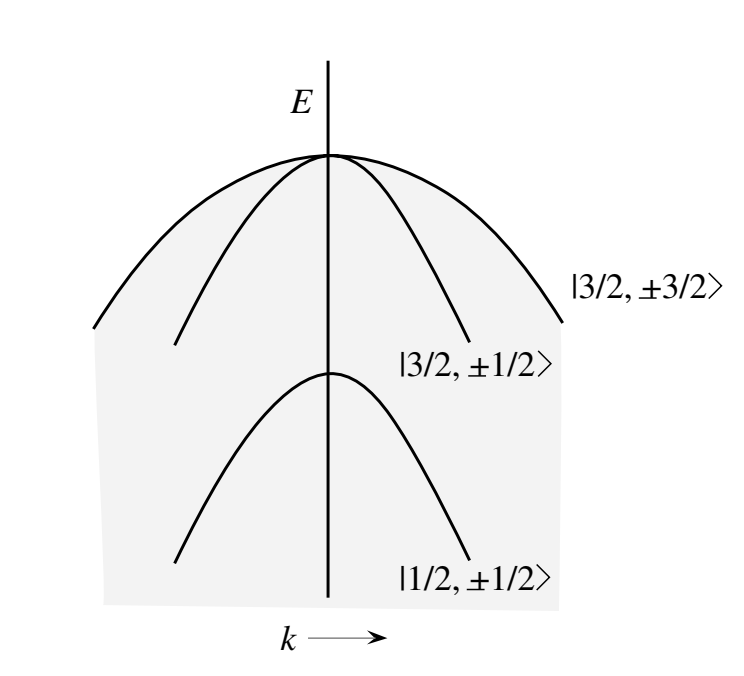
\includegraphics[width=\textwidth]{img/valence_bandstructure.png}
		\\[0.5em]
		\refstepcounter{figure}
		\textbf{Figure~\thefigure.} The general form of the valence bandstructure after incorporating spin--orbit coupling. At the Brillouin zone center ($\mathbf{k} = 0$), the electronic states exhibit well-defined angular momentum character.
		\label{fig:valence_bandstructure}
	\end{minipage}%
	\hfill
	\begin{minipage}{0.48\textwidth}
		\centering
		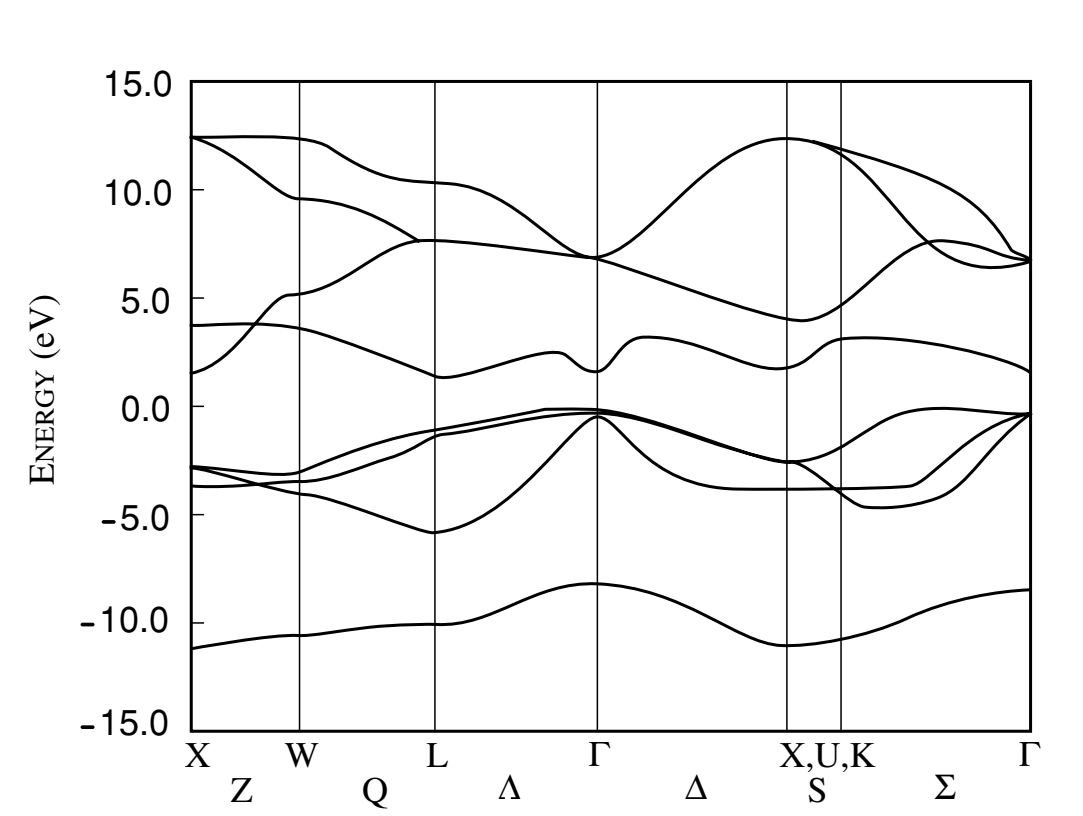
\includegraphics[width=\textwidth]{img/GaAs-spinorbit.png}
		\\[0.5em]
		\refstepcounter{figure}
		\textbf{Figure~\thefigure.} Tight-binding bandstructure of GaAs computed with spin--orbit coupling included. The degeneracy between the light-hole, heavy-hole, and split-off bands is lifted as a result of the spin--orbit interaction.
		\label{fig:GaAs_spin_orbit}
	\end{minipage}
\end{figure}


\subsection{Symmetry of Bandedge States}
In direct bandgap semiconductors, the conduction band minimum occurs at the \( \Gamma \)-point. The periodic part of the Bloch wavefunction at this point is spherically symmetric and primarily composed of \( s \)-type atomic orbitals. As one moves away from the band edge, the eigenstates acquire increasing contributions from \( p \)-type orbitals. However, the dominant \( s \)-character near the conduction band edge gives rise to important optical transition selection rules, which will be discussed in more detail later.

In contrast, indirect bandgap semiconductors such as silicon and germanium exhibit conduction band minima away from the \( \Gamma \)-point. In silicon, the minimum lies near the \( X \)-point and is six-fold degenerate, while in germanium it occurs at the \( L \)-point. The electronic states at these minima are highly anisotropic and involve complex combinations of \( s \)- and \( p \)-type orbitals (\( p_x \), \( p_y \), and \( p_z \)) in their wavefunction composition.

Despite the differences in conduction band behavior, the valence band edge structure in most semiconductors is qualitatively similar. The periodic component of the wavefunction at the valence band maximum is primarily \( p \)-type, which enhances the influence of spin–orbit coupling in this region.

In the absence of spin–orbit interaction, the top of the valence band is three-fold degenerate (six-fold when spin degeneracy is included). When spin–orbit coupling is taken into account, this degeneracy is lifted, resulting in a four-fold degenerate manifold at the top of the valence band and a lower two-fold degenerate split-off band. The upper four-fold degenerate states comprise the heavy hole (HH) and light hole (LH) bands, while the lower-lying two-fold degenerate states form the split-off band.
\subsection*{Heavy hole states}
\begin{equation}
	\boxed{
		\Phi_{3/2, +3/2} = -\frac{1}{\sqrt{2}} \left( |p_x\rangle + i |p_y\rangle \right) |\uparrow\rangle
	}
\end{equation}

\begin{equation}
	\boxed{
		\Phi_{3/2, -3/2} = \frac{1}{\sqrt{2}} \left( |p_x\rangle - i |p_y\rangle \right) |\downarrow\rangle
	}
\end{equation}

\subsection*{Light hole states}
\begin{equation}
	\boxed{
		\Phi_{3/2, +1/2} = -\frac{1}{\sqrt{6}} \left[ \left( |p_x\rangle + i |p_y\rangle \right) |\downarrow\rangle - 2 |p_z\rangle |\uparrow\rangle \right]
	}
\end{equation}

\begin{equation}
	\boxed{
		\Phi_{3/2, -1/2} = \frac{1}{\sqrt{6}} \left[ \left( |p_x\rangle - i |p_y\rangle \right) |\uparrow\rangle + 2 |p_z\rangle |\downarrow\rangle \right]
	}
\end{equation}

\subsection*{Split-off hole states}
\begin{equation}
	\boxed{
		\Phi_{1/2, +1/2} = -\frac{1}{\sqrt{3}} \left[ \left( |p_x\rangle + i |p_y\rangle \right) |\downarrow\rangle + |p_z\rangle |\uparrow\rangle \right]
	}
\end{equation}

\begin{equation}
	\boxed{
		\Phi_{1/2, -1/2} = \frac{1}{\sqrt{3}} \left[ \left( |p_x\rangle - i |p_y\rangle \right) |\uparrow\rangle + |p_z\rangle |\downarrow\rangle \right]
	}
\end{equation}

\begin{center}
	\begin{minipage}{0.9\textwidth}
		\centering
		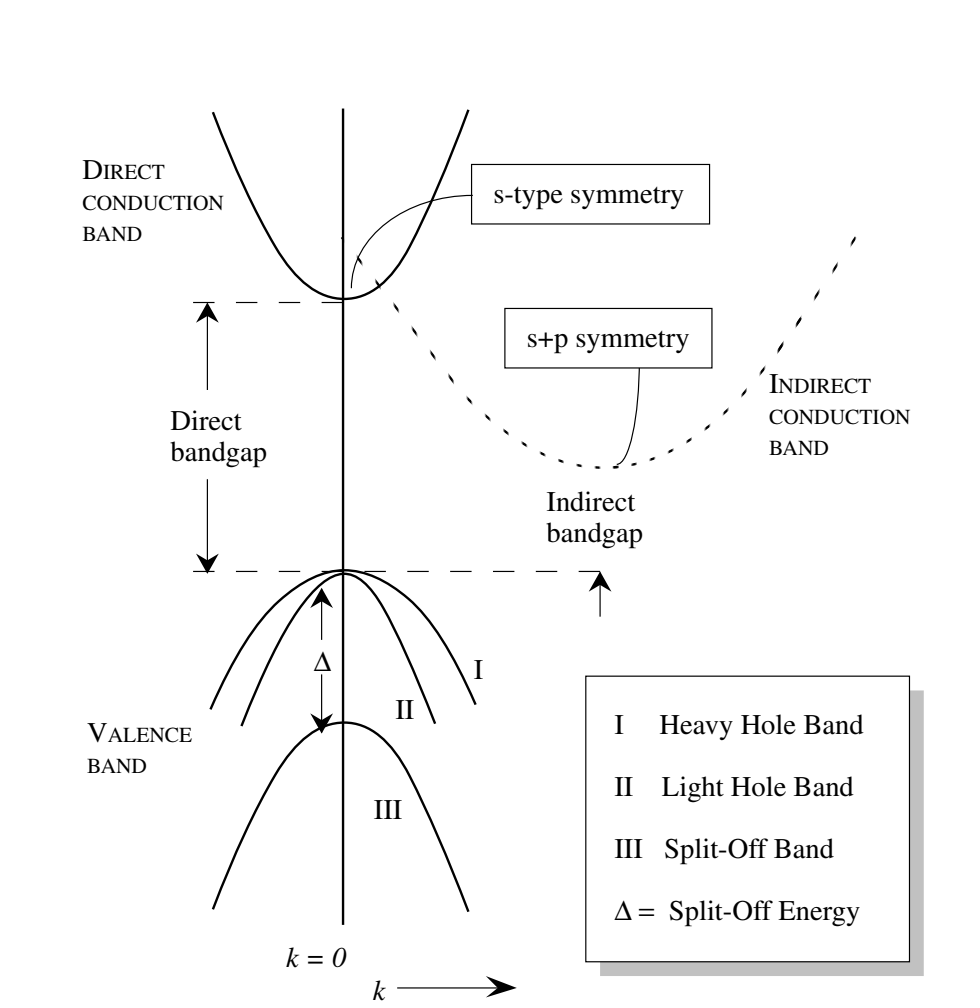
\includegraphics[width=\textwidth]{img/general_valenceband.png}
		\\[0.5em]
		\refstepcounter{figure}
		\textbf{Figure~\thefigure.} Schematic of the valence band and conduction bands in direct and indirect bandgap semiconductors. Solid and dashed lines represent the conduction bands of direct and indirect materials, respectively.
		\label{fig:general_valenceband}
	\end{minipage}
\end{center}

\section{Selected Bandstructures}
\subsection{Silicon}
Silicon forms the foundational material of the modern electronics industry. A key feature of silicon is that it possesses an indirect bandgap, which significantly limits its usefulness in optical applications—particularly for light-emitting devices.\\
The conduction band minimum in silicon does not occur at the \( \Gamma \)-point, but rather near the \( X \)-point in the Brillouin zone, approximately at \( (2\pi/a)(0.85, 0, 0) \). There are six equivalent \( X \)-points in the Brillouin zone, leading to six degenerate conduction band valleys. As a result, the conduction band edge in silicon exhibits a multi-valley structure.\\
Near the conduction band edge, the periodic part of the Bloch wavefunctions exhibits a strong mixture of \( s \)- and \( p \)-type character. Specifically, along the longitudinal direction (aligned with the valley axis, e.g., the \( x \)-axis for the [100] valley), the states have contributions from \( s \)- and \( p_x \)-type orbitals. In the transverse directions (\( y \) and \( z \)), the wavefunction is composed primarily of \( p_y \)- and \( p_z \)-like components.\\
Close to the band edge, the energy dispersion relation can be approximated by an ellipsoidal form. For a given valley aligned along the [100] direction, the energy as a function of wavevector \( \mathbf{k} \) is given by:
\begin{equation}
	E(\mathbf{k}) = \frac{\hbar^2 k_x^2}{2 m_l^*} + \frac{\hbar^2}{2 m_t^*} \left( k_y^2 + k_z^2 \right)
\end{equation}
\noindent
Here, \( m_l^* \) is the effective mass along the longitudinal axis of the ellipsoid (parallel to the valley direction), and \( m_t^* \) is the effective mass in the transverse directions. This anisotropic mass behavior reflects the ellipsoidal constant-energy surfaces around each conduction band minimum.
\begin{center}
	\begin{minipage}{0.7\textwidth}
		\centering
		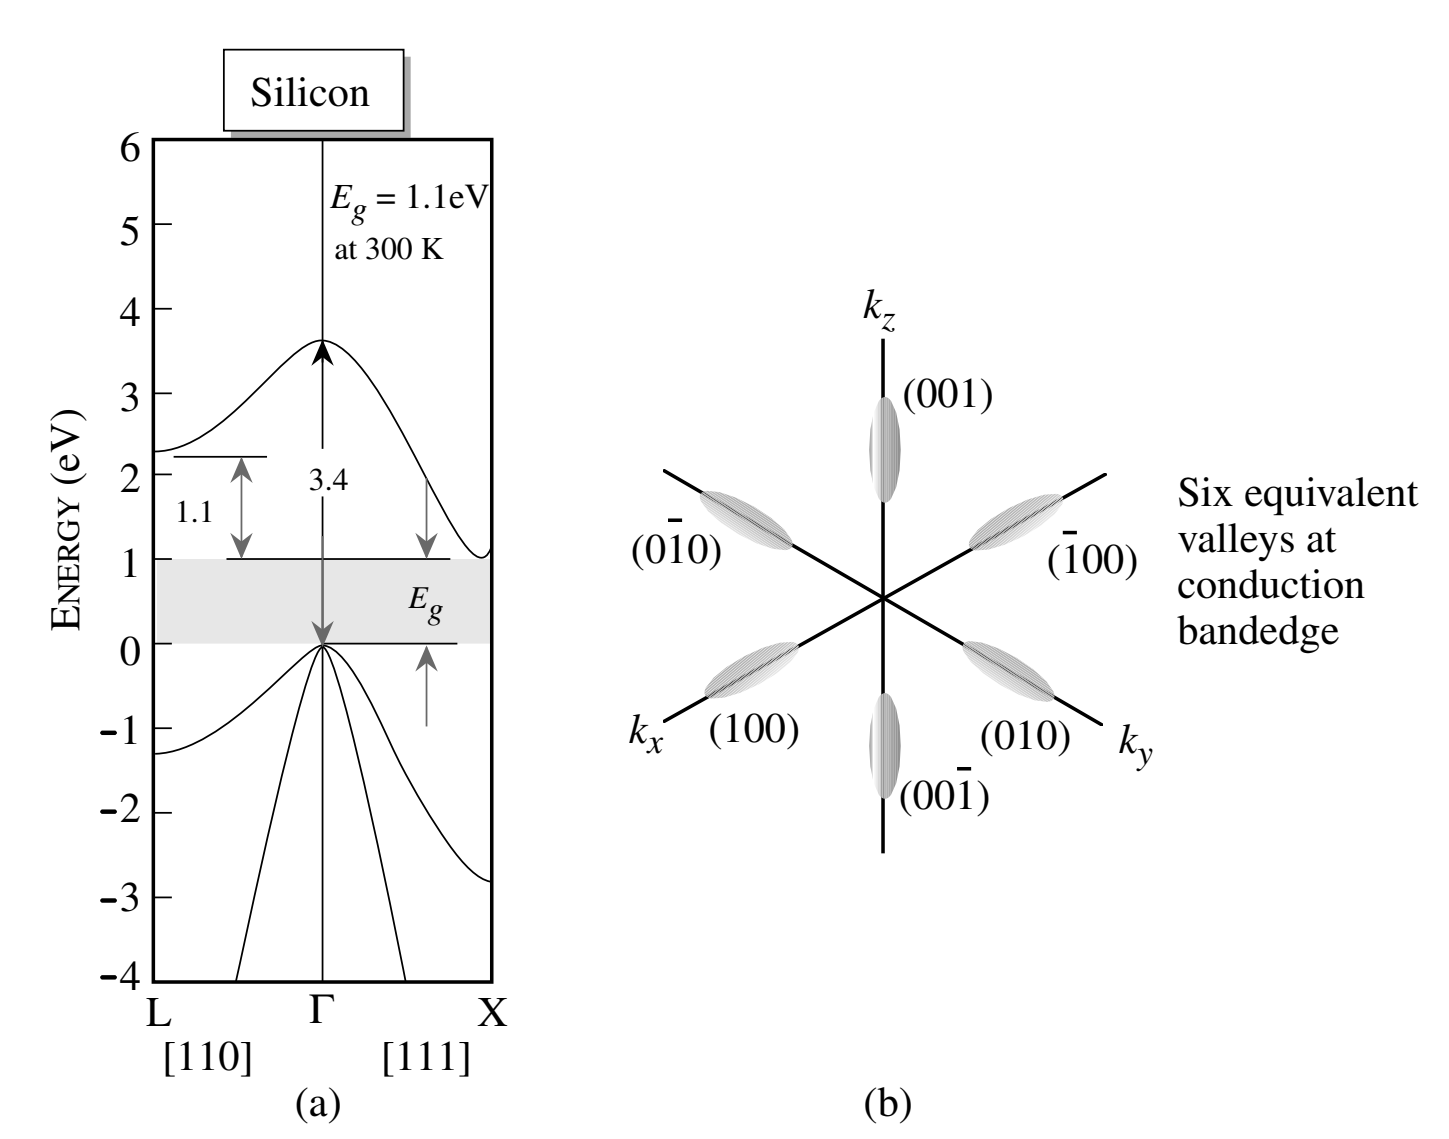
\includegraphics[width=\textwidth]{img/silicon.png}
		\\[0.5em]
		\refstepcounter{figure}
		\textbf{Figure~\thefigure.}
		\label{fig:Silicon}
	\end{minipage}
\end{center}

\subsection{GaAs}
The bandstructure near the band edge in GaAs is characterized by a direct bandgap located at the \( \Gamma \)-point. This direct bandgap is one of the key reasons for the technological relevance of GaAs, as it enables excellent optical properties and high electron mobility in the conduction band.\\
Near the conduction band minimum at \( \Gamma \), the energy-momentum relationship can be approximated by the simple parabolic form:
\begin{equation*}
	E = \frac{\hbar^2 k^2}{2 m^*}
\end{equation*}
\noindent
with an effective mass \( m^* = 0.067 m_0 \), where \( m_0 \) is the free electron mass.\\
A more accurate representation, especially at higher energies, is provided by the nonparabolic dispersion relation:
\begin{equation*}
	E(1 + \alpha E) = \frac{\hbar^2 k^2}{2 m^*}
\end{equation*}
\noindent
where the nonparabolicity parameter \( \alpha \) has a value of approximately \( 0.67\, \text{eV}^{-1} \).\\
For high electric field transport, it is important to consider higher energy conduction band valleys. Above the \( \Gamma \)-valley lie the \( L \)-valleys. There are eight equivalent \( L \)-points in the Brillouin zone, but due to equivalence under reciprocal lattice translations, only four of these are distinct. The energy separation between the \( \Gamma \) minimum and the \( L \)-valleys is approximately \( \Delta E_{\Gamma L} = 0.29\, \text{eV} \). The effective mass in the \( L \)-valley is significantly larger than at \( \Gamma \), with:
\begin{equation}
	m^*_{L} \approx 0.25\, m_0
\end{equation}
This mass difference plays a crucial role in high-field transport behavior, including the onset of negative differential resistance. At still higher energies lies the \( X \)-valley, separated from \( \Gamma \) by approximately \( \Delta E_{\Gamma X} \approx 0.58\, \text{eV} \). The effective mass in the \( X \)-valley is also large:
\begin{equation}
	m^*_{X} \approx 0.6\, m_0
\end{equation}
Under high electric fields, electrons can be transferred from the \( \Gamma \)-valley into the higher-energy \( L \) and \( X \) valleys, making these regions of the conduction band particularly important for transport properties.\\
The valence band in GaAs exhibits the standard structure consisting of heavy hole (HH), light hole (LH), and split-off (SO) bands. Due to the relatively large spin–orbit splitting in GaAs, the SO band lies significantly lower in energy and generally does not contribute to electronic or optoelectronic processes under typical operating conditions.\\
The valence band structure can be described using the Kohn–Luttinger parameters for GaAs, which are:
\begin{align*}
	\gamma_1 & = 6.85 \\
	\gamma_2 & = 2.10 \\
	\gamma_3 & = 2.90
\end{align*}
These parameters yield the following density-of-states effective masses for holes:
\begin{align*}
	m^*_{\text{HH}} & = 0.45\, m_0 \\
	m^*_{\text{LH}} & = 0.08\, m_0
\end{align*}
As with silicon, the hole effective masses in GaAs are highly anisotropic, and the \( E(\mathbf{k}) \) relation for holes reflects this anisotropy in both curvature and carrier dynamics.
\begin{figure}[h!]
	\centering
	\begin{minipage}{0.36\textwidth}
		\centering
		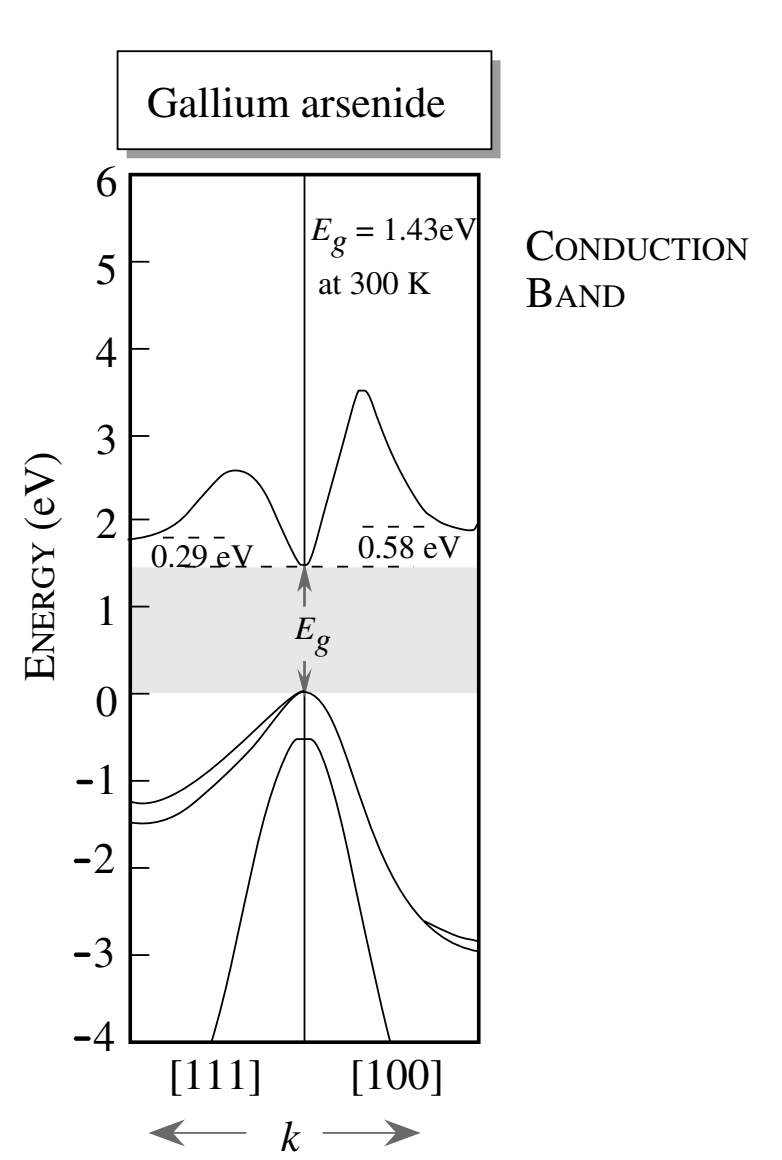
\includegraphics[width=\textwidth]{img/Gallium.png}
		\\[0.5em]
		\refstepcounter{figure}
		\textbf{Figure~\thefigure.}
		\label{fig:Gallium}
	\end{minipage}%
	\hfill
	\begin{minipage}{0.64\textwidth}
		\centering
		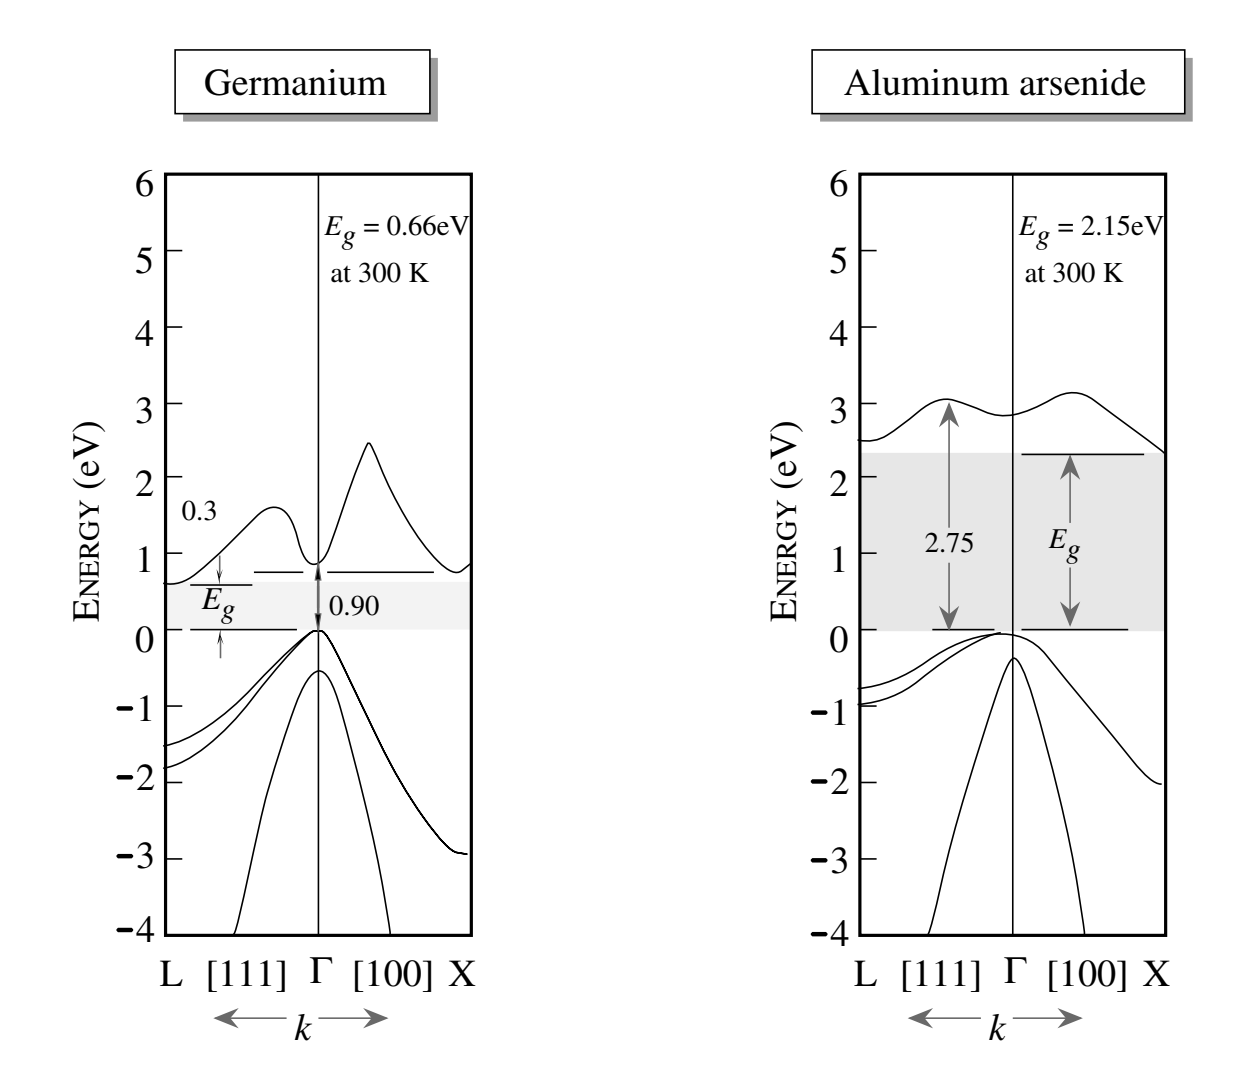
\includegraphics[width=\textwidth]{img/Germanium&Aluminium.png}
		\\[0.5em]
		\refstepcounter{figure}
		\textbf{Figure~\thefigure.}
		\label{fig:Germanium&Aluminium}
	\end{minipage}
\end{figure}

\begin{center}
	\begin{minipage}{0.7\textwidth}
		\centering
		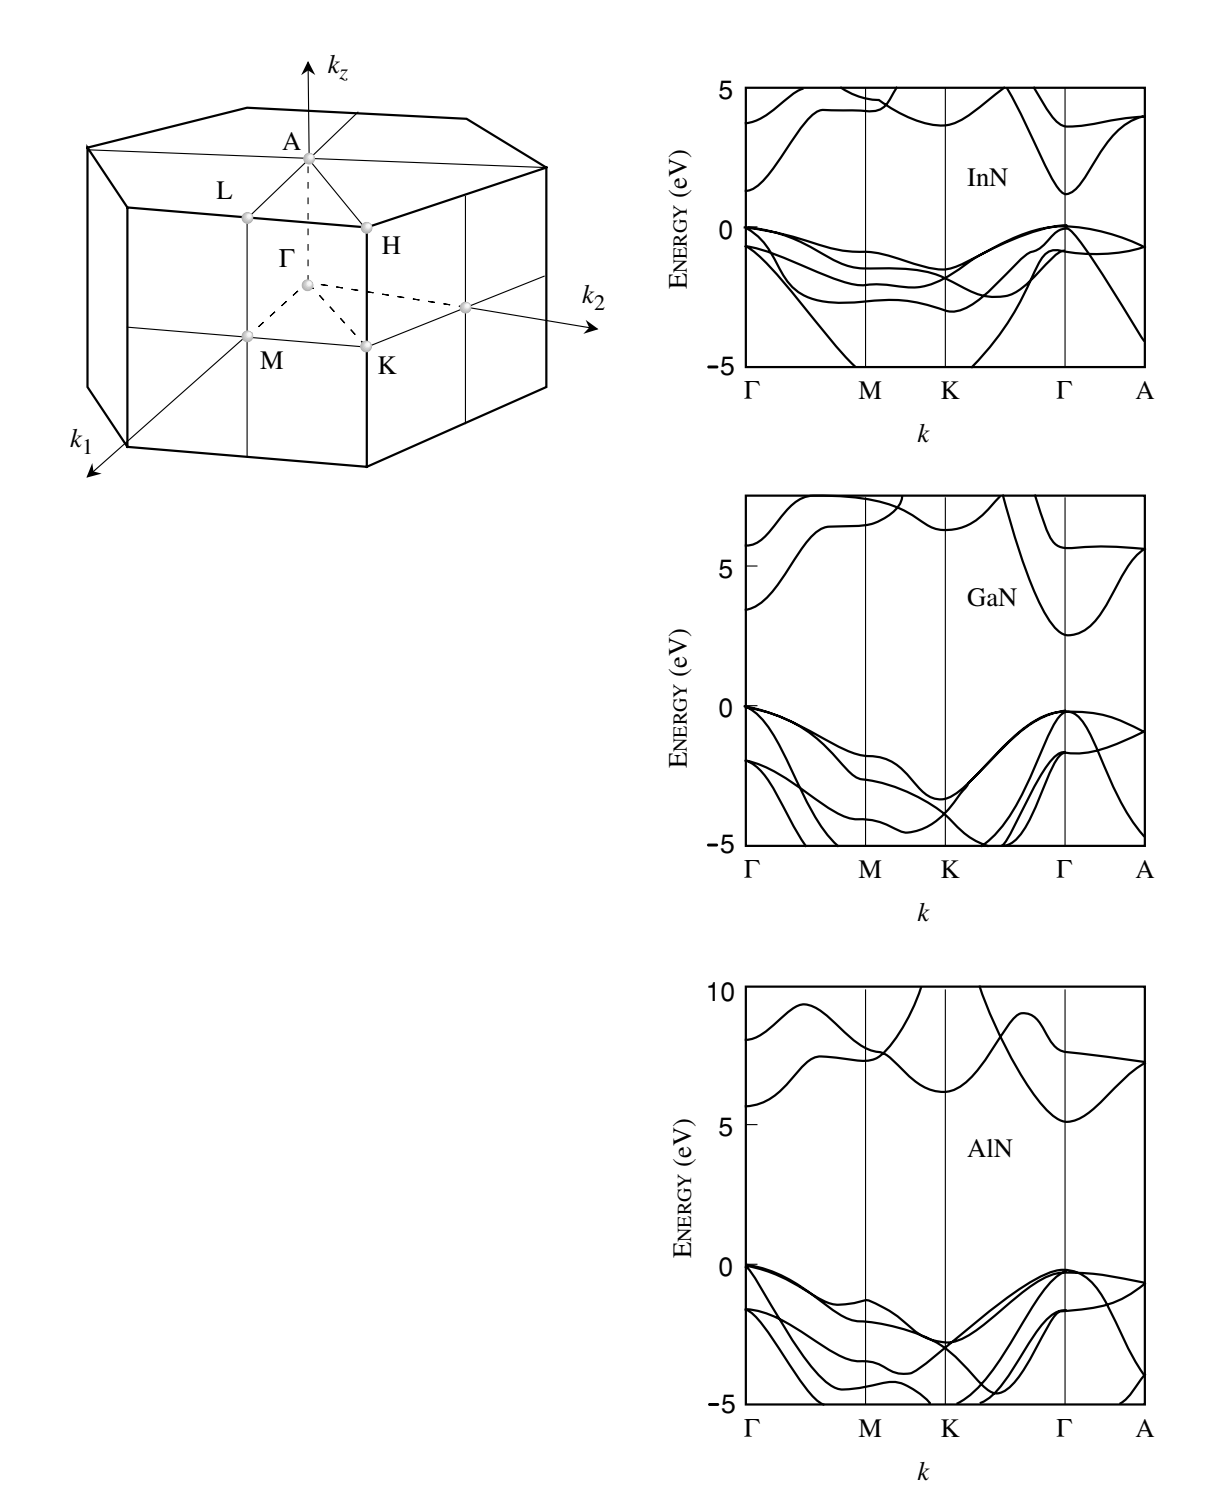
\includegraphics[width=\textwidth]{img/bandstructure_materials.png}
		\\[0.5em]
		\refstepcounter{figure}
		\textbf{Figure~\thefigure.}  Bandstructure of InN, GaN, and AlN. Also shown is the Brillioun zone.
		\label{fig:bandstructure_materials}
	\end{minipage}
\end{center}


\section{Mobile Carriers: Intrinsic Carriers}
In metals, the density of mobile charge carriers is extremely high, typically on the order of \( \sim 10^{23}~\text{cm}^{-3} \). In contrast, a semiconductor with a completely filled valence band and an empty conduction band does not conduct current under equilibrium conditions.

However, if electrons are excited from the valence band into the conduction band—either thermally or through doping—then two types of mobile charge carriers can exist. The electrons promoted to the conduction band contribute to conduction, and the absence of electrons (i.e., holes) left behind in the valence band also behave as positively charged mobile carriers.

If the concentration of conduction band electrons is denoted by \( n \), and the concentration of holes in the valence band is \( p \), then the total mobile carrier concentration in the material is given by:

\begin{equation}
	n_{\text{total}} = n + p
\end{equation}
In a three-dimensional semiconductor, the density of states (DOS) in the conduction band is given by:
\begin{equation}
	N(E) = \frac{\sqrt{2} \left( m^*_{\text{dos}} \right)^{3/2} \left( E - E_c \right)^{1/2}}{\pi^2 \hbar^3}
\end{equation}
\noindent
where:
\begin{itemize}
	\item \( N(E) \) is the density of available electronic states per unit volume per unit energy,
	\item \( m^*_{\text{dos}} \) is the effective density of states mass for the conduction band,
	\item \( E_c \) is the conduction band edge.
\end{itemize}

\begin{center}
	\begin{minipage}{0.8\textwidth}
		\centering
		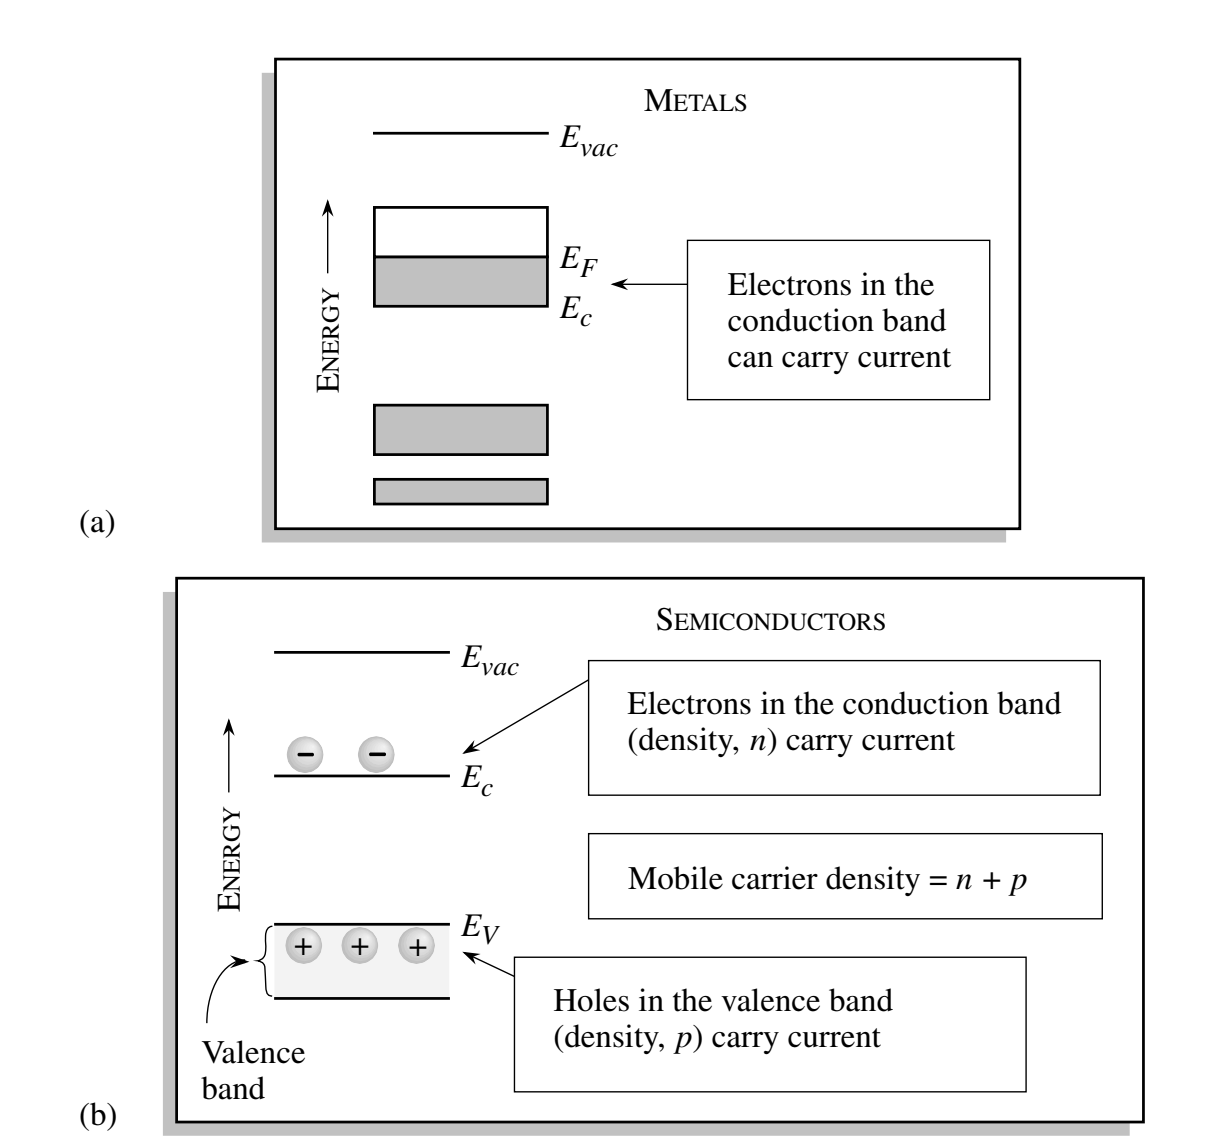
\includegraphics[width=\textwidth]{img/scheme_allowed_energy.png}
		\\[0.5em]
		\refstepcounter{figure}
		\textbf{Figure~\thefigure.}  (a) Schematic of allowed energy bands in a metal. Electrons in the highest partially filled band contribute to electrical conduction.
		(b) Energy band diagram of a typical semiconductor, where current is carried by electrons in the conduction band and holes in the valence band.
		\label{fig:allowed_energy_bands}
	\end{minipage}
\end{center}

In direct bandgap semiconductors, the density of states effective mass \( m^*_{\text{dos}} \) for the conduction band is simply equal to the electron effective mass at the band minimum. However, in indirect bandgap semiconductors, \( m^*_{\text{dos}} \) is defined as the geometric mean of the effective masses along the three principal axes:
\begin{equation}
	m^*_{\text{dos}} = \left( m_1^* m_2^* m_3^* \right)^{1/3}
\end{equation}
\noindent
where \( m_1^*, m_2^*, m_3^* \) are the effective masses along the principal crystallographic directions. For silicon, which has six equivalent \( X \)-valleys, this becomes:
\begin{equation}
	m^*_{\text{dos}} = 6 \left( m_t^2 m_l \right)^{1/3}
\end{equation}
\noindent
where \( m_l \) and \( m_t \) are the longitudinal and transverse effective masses of the conduction band ellipsoids, respectively.

For the valence band, which consists of heavy hole (HH) and light hole (LH) bands, the effective density of states mass can be approximated by:
\begin{equation}
	m^*_{\text{dos}} = \left( m_{\text{hh}}^{*3/2} + m_{\text{lh}}^{*3/2} \right)^{2/3}
\end{equation}

In intrinsic semiconductors, conduction band electrons originate from the valence band, and thus the electron and hole densities are equal:
\begin{equation*}
	n = p = n_i = p_i
\end{equation*}
The electron concentration in the conduction band is given by the integral:
\begin{equation}
	n = \int_{E_c}^{\infty} N_e(E) f(E) \, dE
\end{equation}
\noindent
Using the expression for the density of states and the Fermi-Dirac distribution, this becomes:
\begin{equation}
	n = \frac{1}{2\pi^2} \left( \frac{2 m_e^*}{\hbar^2} \right)^{3/2} \int_{E_c}^{\infty} \frac{(E - E_c)^{1/2}}{1 + \exp\left( \frac{E - E_F}{k_B T} \right)} \, dE
\end{equation}
\noindent
In the non-degenerate limit, where \( (E - E_F) \gg k_B T \), we can approximate the Fermi-Dirac function by the Boltzmann distribution, and the integral simplifies to:
\begin{equation}
	n = N_c \exp \left( \frac{E_F - E_c}{k_B T} \right)
\end{equation}
\noindent
where the effective density of states in the conduction band is:
\begin{equation}
	N_c = 2 \left( \frac{m_e^* k_B T}{2\pi \hbar^2} \right)^{3/2}
\end{equation}
A similar result holds for the hole concentration:
\begin{equation}
	p = N_v \exp \left( \frac{E_v - E_F}{k_B T} \right)
\end{equation}
\noindent
where:
\begin{equation}
	N_v = 2 \left( \frac{m_h^* k_B T}{2\pi \hbar^2} \right)^{3/2}
\end{equation}

The product \( np \) is independent of the Fermi level and depends only on temperature and intrinsic material properties:
\begin{equation}
	np = N_c N_v \exp \left( \frac{-E_g}{k_B T} \right)
\end{equation}
\noindent
This result is known as the \textit{law of mass action}. If \( n \) increases, \( p \) must decrease accordingly to maintain this constant product, and vice versa.

For an intrinsic semiconductor, where \( n = p = n_i \), we can express the intrinsic carrier concentration as:
\begin{equation}
	n_i = p_i = 2 \left( \frac{k_B T}{2\pi \hbar^2} \right)^{3/2} \left( m_e^* m_h^* \right)^{3/4} \exp \left( \frac{-E_g}{2k_B T} \right)
\end{equation}
Additionally, the intrinsic Fermi level \( E_i \) is approximately given by:
\begin{equation}
	E_i = \frac{E_c + E_v}{2} + \frac{3}{4} k_B T \ln \left( \frac{m_h^*}{m_e^*} \right)
\end{equation}
In computing the density of states masses \( m_e^* \) and \( m_h^* \), one must account for the number of equivalent conduction band valleys and the contributions from both heavy and light hole bands in the valence band.
\begin{center}
	\begin{minipage}{0.9\textwidth}
		\centering
		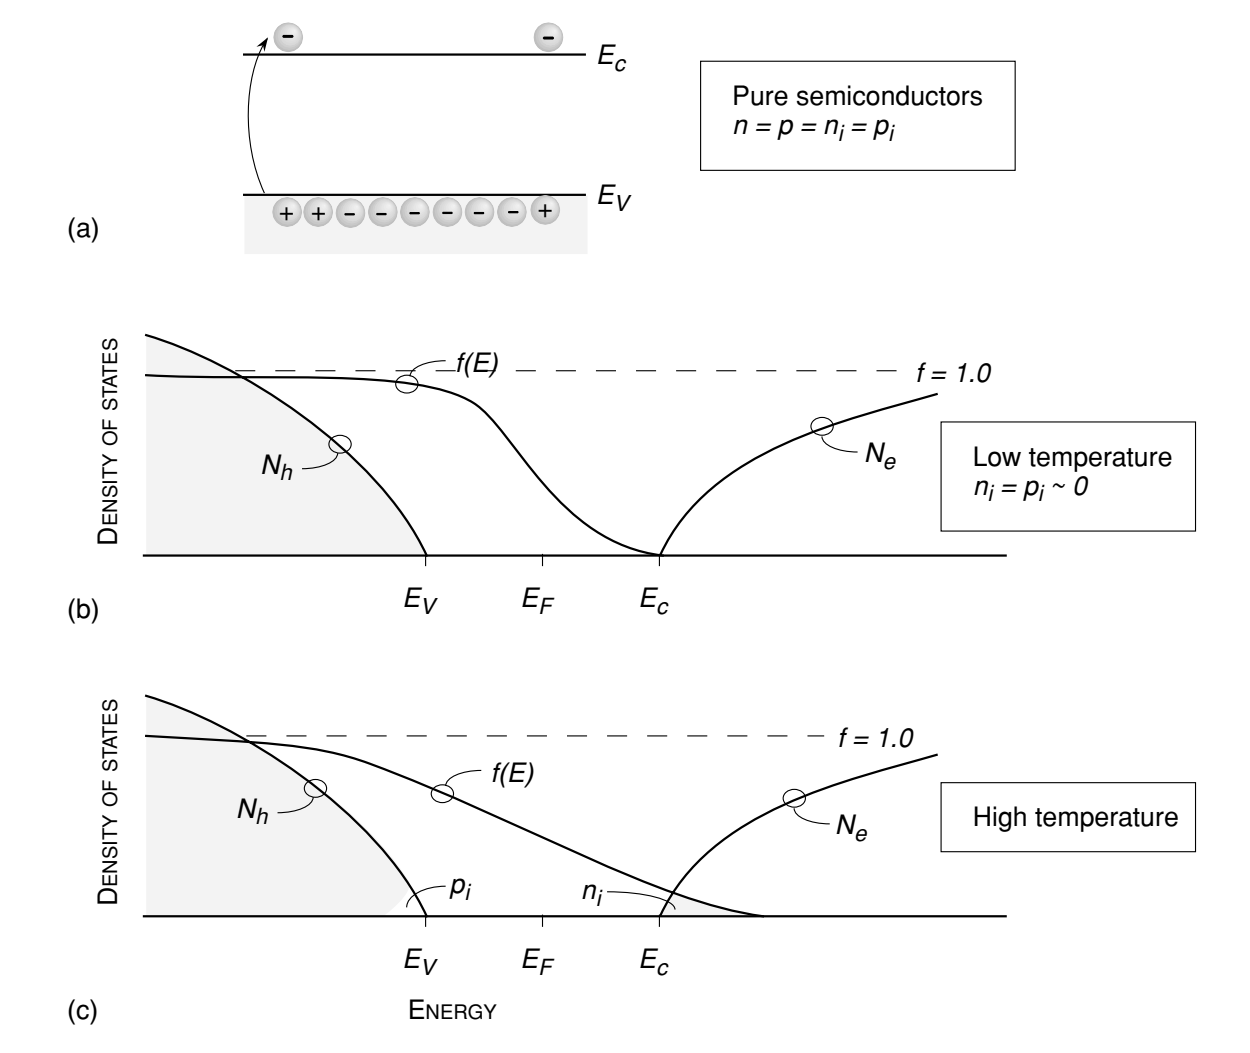
\includegraphics[width=\textwidth]{img/hole_denisties&Fermi_occupation.png}
		\\[0.5em]
		\refstepcounter{figure}
		\textbf{Figure~\thefigure.}
		(a) Illustration of equal electron and hole concentrations in an intrinsic (pure) semiconductor.
		(b) Density of states and Fermi-Dirac distribution at low temperature.
		(c) Density of states and Fermi function at high temperature, where intrinsic carrier concentrations $n_i$ and $p_i$ increase significantly.
		\label{fig:hole_denisties&Fermi_occupation}
	\end{minipage}
\end{center}

\section{Doping: Donors and Acceptors}
There are two primary types of dopants in semiconductors: \textit{donors}, which contribute electrons to the conduction band, and \textit{acceptors}, which accept electrons from the valence band, thereby creating holes. To understand how donor and acceptor states arise, consider a donor atom substituted into a crystal lattice.\\
For example, in silicon, a typical donor is a group V (pentavalent) atom that replaces a Si atom. Four of the donor's valence electrons form covalent bonds with neighboring Si atoms, just as in a normal Si lattice. The fifth valence electron, however, is left loosely bound. It experiences an attractive force from the now positively charged donor ion, which has a net charge of \( +e \). This interaction is Coulombic in nature but is screened by the dielectric constant \( \varepsilon \) of the semiconductor:
\begin{equation}
	U(r) = -\frac{e^2}{4\pi \varepsilon r}
\end{equation}
\noindent
where \( \varepsilon = \varepsilon_0 \varepsilon_r \), the product of vacuum permittivity and the relative dielectric constant of the material.\\
This scenario closely resembles the hydrogen atom problem, but with two modifications: the electron has an effective mass \( m^* \) rather than the free electron mass, and the Coulomb potential is reduced by the dielectric screening. The ground-state energy of the donor-bound electron is then given by:
\begin{equation}
	E_d = E_c - \frac{m^* e^4}{2(4\pi \varepsilon)^2 \hbar^2}
	= E_c - 13.6\,\text{eV} \left( \frac{m^*}{m_0} \right) \left( \frac{1}{\varepsilon_r^2} \right)
\end{equation}
\noindent
where \( E_c \) is the conduction band edge, and \( m_0 \) is the free electron mass.
In contrast to the hydrogen atom, where the energy level is referenced to the vacuum, in semiconductors, the donor energy is referenced from the conduction band edge. The effective mass \( m^* \) used in this calculation is the conductivity effective mass \( m^*_\sigma \), which reflects how electrons respond to external fields. This mass also governs donor binding energies and charge transport.\\
For direct bandgap semiconductors such as GaAs, the conductivity mass is simply the electron effective mass at the conduction band minimum. In indirect semiconductors like silicon, the conductivity mass is given by:
\begin{equation}
	{m^*_\sigma} = 3\left( \frac{1}{m_l^*} + \frac{2}{m_t^*} \right)^{-1}
\end{equation}
\noindent
where \( m_l^* \) and \( m_t^* \) are the longitudinal and transverse effective masses of the conduction band valleys.\\
\begin{figure}[h!]
	\centering
	\begin{minipage}{0.44\textwidth}
		\centering
		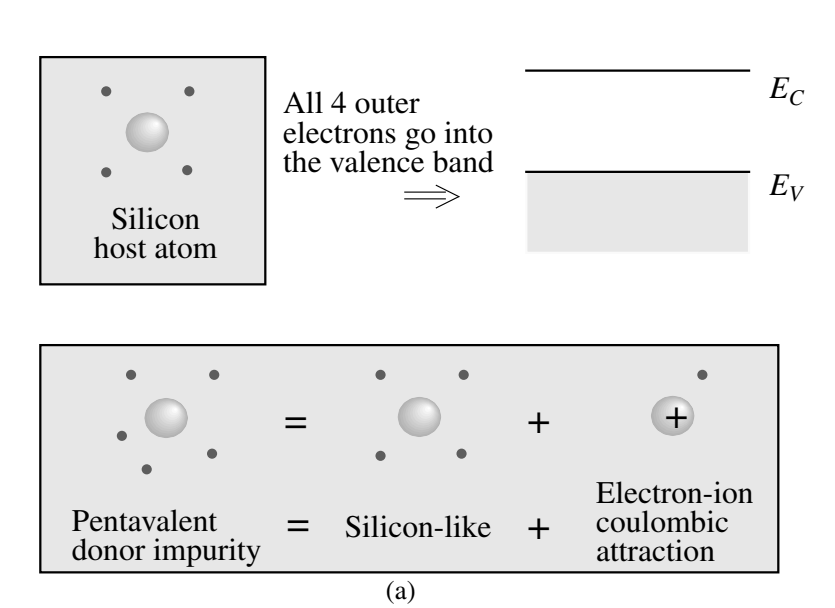
\includegraphics[width=\textwidth]{img/donors&acceptors.png}
		\\[0.5em]
		\refstepcounter{figure}
		\textbf{Figure~\thefigure.} \small Schematic illustrating the donor model in semiconductors. The problem is approached by considering the host atom plus a Coulomb interaction. Silicon contributes four valence electrons per atom. A donor atom provides five electrons, four of which fill the valence band, while the fifth can be thermally excited into the conduction band.
		\label{fig:donors&acceptors}
	\end{minipage}%
	\hfill
	\begin{minipage}{0.52\textwidth}
		\centering
		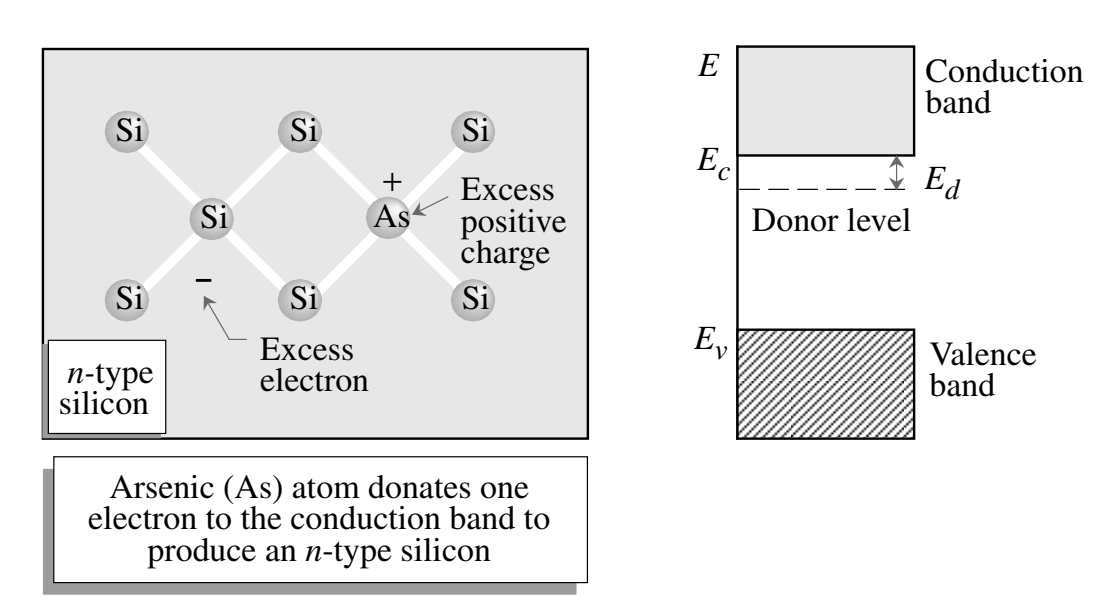
\includegraphics[width=\textwidth]{img/SiAs.png}
		\\[0.5em]
		\refstepcounter{figure}
		\textbf{Figure~\thefigure.} \small Charge distribution around an arsenic impurity in silicon. Arsenic, with five valence electrons, forms four covalent bonds like silicon, while the fifth electron remains free for conduction. Upon ionization, the arsenic atom donates this electron to the conduction band and acts as a donor.
		\label{fig:SiAs}
	\end{minipage}
\end{figure}
According to this simplified model, the donor binding energy depends only on the properties of the host material—namely, its dielectric constant \( \varepsilon_r \) and effective mass \( m^* \)—and not on the specific dopant species. Using this model, typical donor binding energies are:
\begin{itemize}
	\item Germanium (Ge): \( \sim 0.006\,\text{eV} \)
	\item Silicon (Si): \( \sim 0.025\,\text{eV} \)
	\item Gallium Arsenide (GaAs): \( \sim 0.007\,\text{eV} \)
\end{itemize}
In practice, small deviations from these values occur due to simplifications in the model. The discrepancy arises from local modifications in the potential near the impurity site—known as the \textit{central cell correction}—which slightly perturbs the donor energy levels beyond what is predicted by the hydrogenic approximation.\\
Acceptors represent another class of intentional impurities. Like donors, they introduce localized energy levels in the bandgap. An acceptor is neutral when unoccupied and negatively charged when it captures an electron from the valence band, leaving behind a mobile hole. These levels are created by substituting host atoms with impurities that have one fewer valence electron. For example, group III elements act as acceptors in group IV semiconductors such as Si and Ge, while Si can act as an acceptor in GaAs if it replaces an As atom.\\
Thus, donors and acceptors serve to modulate the free carrier concentrations in semiconductors, enabling control over electronic and optoelectronic behavior.

\subsection{Carriers in Doped Semiconductors}
As previously discussed, introducing a donor atom into a semiconductor can, in principle, contribute an extra electron to the conduction band. However, whether this electron becomes a free carrier or remains bound to the donor site depends on several factors: the donor binding energy, the donor concentration, and the temperature.\\
At very low temperatures, donor electrons typically remain bound to their parent atoms. This phenomenon, known as \textit{carrier freezeout}, results in minimal free carrier concentration and hence poor conductivity. As the temperature increases, thermal energy becomes sufficient to ionize donor electrons, which then occupy states in the conduction band and act as mobile charge carriers. These free electrons significantly affect the electrical conductivity of the material. The donor site, now lacking an electron, becomes a positively charged ion.\\
A similar process occurs for acceptor atoms: when an acceptor captures an electron from the valence band, it becomes negatively charged and creates a mobile hole in the valence band.\\
In general, as discussed before, the relationship between the electron concentration \( n \) and the Fermi level \( E_F \) is given by:
\begin{equation*}
	n = \int_{E_c}^\infty N(E) f(E) \, dE
\end{equation*}
\noindent
This equation must usually be solved numerically. However, a useful analytical approximation is provided by the \textit{Joyce–Dixon} formula. According to this approximation, the Fermi level is related to the carrier concentration as follows:
\begin{equation}
	E_F = E_c + k_B T \ln \left( \frac{n}{N_c} \right) + \frac{k_B T}{\sqrt{8}} \left( \frac{n}{N_c} \right)
\end{equation}
\noindent
Alternatively, for hole concentration \( p \), the expression becomes:
\begin{equation}
	E_F = E_v - k_B T \ln \left( \frac{p}{N_v} \right) - \frac{k_B T}{\sqrt{8}} \left( \frac{p}{N_v} \right)
\end{equation}
\noindent
The effective density of states in the conduction band is given by:
\begin{equation*}
	N_c = 2 \left( \frac{m_e^* k_B T}{2\pi \hbar^2} \right)^{3/2}
\end{equation*}
\noindent
and similarly, the valence band effective density of states is:
\begin{equation*}
	N_v = 2 \left( \frac{m_h^* k_B T}{2\pi \hbar^2} \right)^{3/2}
\end{equation*}
These expressions allow one to estimate the Fermi level \( E_F \) for a known carrier concentration \( n \), or vice versa, by iterative methods. If the correction terms \( (n/\sqrt{8}N_c) \) or \( (p/\sqrt{8}N_v) \) are neglected, the equations reduce to the standard Boltzmann approximation:
\begin{equation}
	n \approx N_c \exp \left( \frac{E_F - E_c}{k_B T} \right)
\end{equation}
\noindent
and
\begin{equation}
	p \approx N_v \exp \left( \frac{E_v - E_F}{k_B T} \right)
\end{equation}
This simplified form is valid under non-degenerate conditions, where the Fermi level is several \( k_B T \) away from the band edges.

\subsection{Mobile Carrier Density and Carrier Freezeout}
\begin{center}
	\begin{minipage}{0.7\textwidth}
		\centering
		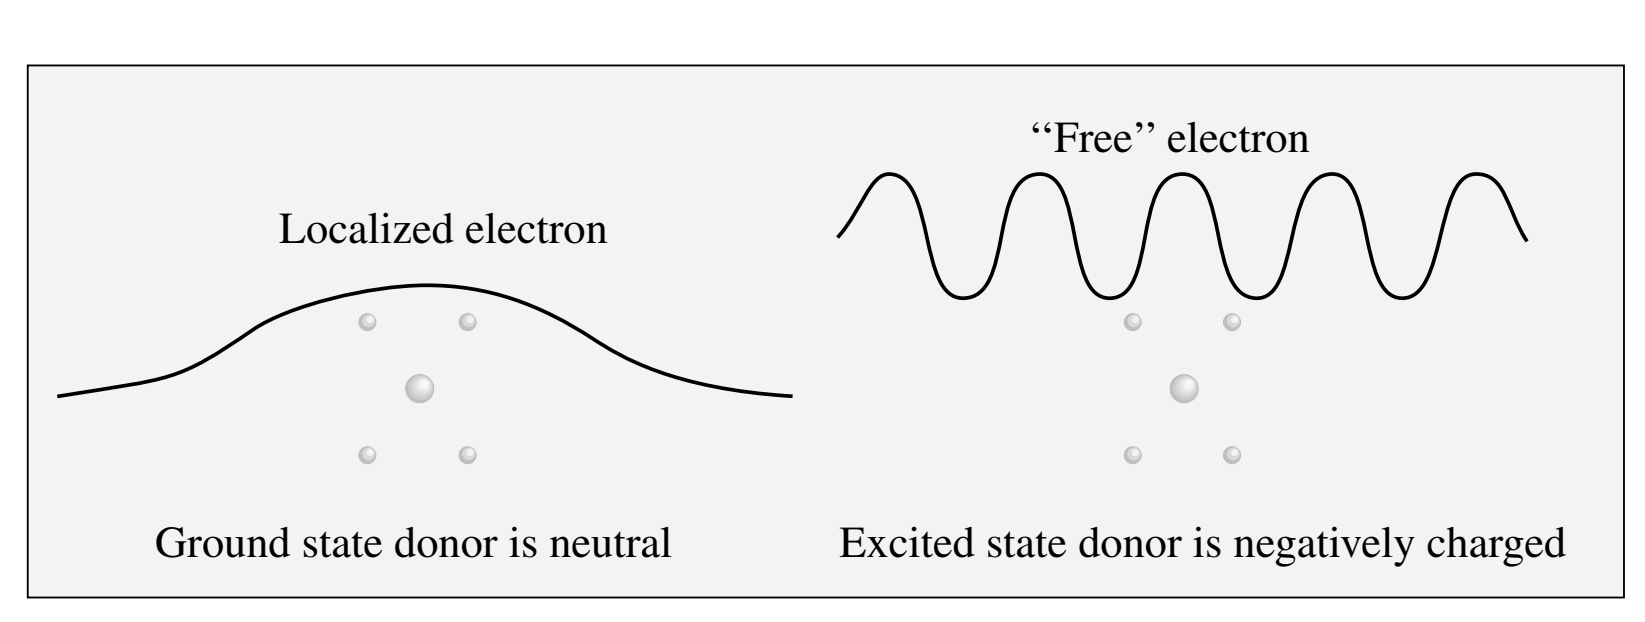
\includegraphics[width=\textwidth]{img/Electron_band.png}
		\\[0.5em]
		\refstepcounter{figure}
		\textbf{Figure~\thefigure.}An electron bound to a donor does not participate in conduction. Only when the donor is ionized does the electron become free and contribute to electrical transport.
		\label{fig:Electron_band}
	\end{minipage}
\end{center}

In the ground state of a donor atom embedded in a semiconductor, the excess electron introduced by the donor is localized near the donor nucleus. Since this bound state does not contribute to electrical conductivity, such electrons are not useful for modifying the electronic properties of the material.\\
At very low temperatures, donor electrons remain bound to the donor atoms—a phenomenon known as \textit{carrier freeze-out}. As the temperature increases, thermal excitation allows the donor electrons to be ionized into the conduction band, where they become mobile and contribute to current transport. The donor atom, once ionized, becomes positively charged and acts as a scattering center for conduction electrons. The detailed analysis of scattering effects will be addressed in a later section.\\
The electron–donor system may exist in the following possible configurations:
\begin{enumerate}
	\item the donor electron is ionized and free in the conduction band;
	\item one electron is bound to the donor atom (with spin-up or spin-down);
	\item two electrons attempt to occupy the donor site.
\end{enumerate}
Although the third case is theoretically possible, the strong Coulombic repulsion between two electrons on the same donor site makes such double occupation energetically prohibitive. Therefore, a donor can bind at most one electron at a time, with either spin orientation.\\
Due to the two available spin states for the bound electron, the donor occupation statistics follow Fermi–Dirac statistics with a factor of two in the numerator. The probability that a donor level at energy \( E_d \) is occupied by an electron is given by:
\begin{equation}
	f_d = \frac{1}{1 + \frac{1}{2} \exp\left( \frac{E_d - E_F}{k_B T} \right)}
\end{equation}
\noindent
where \( E_F \) is the Fermi level, \( k_B \) is Boltzmann’s constant, and \( T \) is the temperature.
The number density of electrons bound to donor sites is therefore:
\begin{equation}
	n_d = N_d \cdot f_d = \frac{N_d}{1 + \frac{1}{2} \exp\left( \frac{E_d - E_F}{k_B T} \right)}
\end{equation}
\noindent
For \( (E_d - E_F) \gg k_B T \), this simplifies to the Boltzmann approximation:
\begin{equation}
	n_d \approx 2 N_d \exp\left( -\frac{E_d - E_F}{k_B T} \right)
\end{equation}
Similarly, for acceptor levels, the probability that a hole is trapped at an acceptor level is given by:
\begin{equation}
	p_a = \frac{N_a}{1 + \frac{1}{4} \exp\left( \frac{E_F - E_a}{k_B T} \right)}
\end{equation}
\noindent
Here, \( E_a \) is the acceptor level energy, and the factor of \( \frac{1}{4} \) arises from the four-fold degeneracy associated with the doubly degenerate valence band and spin.\\
These expressions allow us to estimate the ionization state of donor and acceptor levels as a function of temperature and Fermi energy.


\subsection{Equilibrium Density of Carriers in Doped Semiconductors}
In a doped semiconductor, we may introduce donor atoms, acceptor atoms, or both. To determine the electron and hole concentrations under such conditions, we must consider the occupation functions of free carriers and dopant states. The key constraint that must be satisfied is the \textit{charge neutrality condition}, given by:
\begin{equation}
	n_c + n_d = N_d - N_a + p_v + p_a
\end{equation}
\noindent
where:
\begin{itemize}
	\item \( n_c \) is the density of free electrons in the conduction band,
	\item \( n_d \) is the density of electrons bound to donor atoms,
	\item \( p_v \) is the density of free holes in the valence band,
	\item \( p_a \) is the density of holes bound to acceptor atoms.
\end{itemize}
\noindent
The electron and hole densities depend on the Fermi energy \( E_F \), and hence the neutrality condition, combined with the Fermi–Dirac occupation probabilities, allows us to determine \( E_F \) at a given temperature. In the general case, this requires numerical methods: a trial Fermi level is chosen and adjusted iteratively until the neutrality equation is satisfied.\\
However, in the case of low doping levels—where carrier concentrations are small—the Boltzmann approximation can be applied, allowing for an analytical treatment. Under this approximation, and neglecting the unity in the denominator of the Fermi function, the free electron concentration is given by:
\begin{equation}
	n = N_c \exp\left( -\frac{E_c - E_F}{k_B T} \right)
\end{equation}
\noindent
For electrons bound to donors, we have:
\begin{equation}
	n_d = \frac{N_d}{1 + \frac{1}{2} \exp\left( \frac{E_d - E_F}{k_B T} \right)} \approx \frac{N_d}{2} \exp\left( \frac{E_d - E_F}{k_B T} \right)
\end{equation}
\noindent
Combining these, the total electron concentration becomes:
\begin{equation}
	n = n + n_d = N_c \exp\left( -\frac{E_c - E_F}{k_B T} \right) + \frac{N_d}{2} \exp\left(\frac{E_d - E_F}{k_B T} \right)
\end{equation}
\noindent
Alternatively, this can be rearranged as:
\begin{equation}
	\frac{n_d}{n_d + n_c} = \frac{1}{1 + \frac{N_c}{2 N_d} \exp\left( -\frac{E_c - E_d}{k_B T} \right)}
\end{equation}
For acceptor doping, a similar analysis leads to:
\begin{equation}
	\frac{p_a}{p + p_a} = \frac{1}{1 + \frac{N_v}{4N_a} \exp\left( -\frac{E_a - E_v}{k_B T} \right)}
\end{equation}
\noindent
where:
\begin{itemize}
	\item \( N_c \), \( N_v \) are the effective density of states in the conduction and valence bands, respectively,
	\item \( N_d \), \( N_a \) are the donor and acceptor concentrations,
	\item \( E_c \), \( E_v \), \( E_d \), and \( E_a \) are the band edge and dopant energy levels.
\end{itemize}
These relations provide a way to estimate carrier concentrations and dopant ionization under low doping conditions.

In the Fig.\ref{fig:Electron_band} we show how free electron density varies with temperature in a n-type silicon sample. As temperature increases, the fraction of “ionized” donors starts to increase until all of the donors are ionized and the free carrier density is equal to the donor density. This region is called the saturation region. Eventually, as the temperature is further raised, the carrier density starts to increase because of the intrinsic carrier density exceeding the donor density. At low temperatures the electrons are bound to the donors. This is the freezeout regime. Semiconductor devices usually operate in the satu- ration region where the mobile carrier density is essentially independent of temperature and is approximately equal to the doping density.
Semiconductor devices cannot operate in the high temperature intrinsic regime, since it is not possible to control intrinsic carrier density by applying an external bias. Thus devices cannot be “shut off ” due to the leakage current from intrinsic carriers. High temperature electronics require large bandgap semiconductors for which the upper temperature limit is high.

\subsection{Heavily Doped Semiconductors}
In the theory discussed so far, we have made several important assumptions that are valid only under low doping conditions:
\begin{enumerate}
	\item The bandstructure of the host crystal is assumed to remain unperturbed, such that the bandedge states are still well described by simple parabolic bands.
	\item Dopants are treated as isolated and non-interacting, with their potential modeled as a simple Coulombic potential.
\end{enumerate}
\noindent These assumptions break down as the doping level increases. When the average spacing between impurity atoms becomes comparable to $\sim 100$~\AA, the potential experienced by an impurity electron is significantly influenced by neighboring impurities. This situation is analogous to the transition from isolated atomic levels to energy bands in a crystal. When atoms are far apart, discrete energy levels exist; however, as their separation decreases to a few angstroms, these levels broaden into bands due to interatomic interactions.\\
\noindent Similarly, at high doping levels, impurity states can overlap and form \textit{impurity bands}. In this regime, several additional physical effects arise, altering the electrical and optical properties of the semiconductor. These effects must be considered for a proper understanding of heavily doped semiconductors.
